\documentclass{article}
\usepackage{NotesPackage}
\usepackage{csquotes}
\usepackage[europeanresistors]{circuitikz}
\usepackage[section]{placeins}

\counterwithin{figure}{section}
\counterwithin{table}{section}
\counterwithin{equation}{section}

\title{Analogue Circuits}
\date{September 17, 2019}
\author{Willoughby Seago}

\newcommand{\notesVersion}{1.0}
\newcommand{\notesDate}{04/01/2021}

\begin{document}
    \maketitle
    These are my notes for the \textit{analogue circuits 2} course from the University of Edinburgh School of Engineering, which I took as an optional course from outside the School of Physics.
    When I took this course in the 2019/20 academic year it was taught by Professor Rebecca Cheung\footnote{\url{https://www.eng.ed.ac.uk/about/people/prof-rebecca-cheung}} and Dr David Laurenson\footnote{\url{https://www.eng.ed.ac.uk/about/people/dr-david-laurenson}}.
    These notes are based on the lectures delivered as part of this course, and the notes provided as part of this course.
    The content within is correct to the best of my knowledge but if you find a mistake or just disagree with something or think it could be improved please let me know.
    
    These notes were produced using \LaTeX\footnote{\url{https://www.latex-project.org/}}.
    Graphs where plotted using Python\footnote{\url{https://www.python.org/}}, Matplotlib\footnote{\url{https://matplotlib.org/}}, NumPy\footnote{\url{https://numpy.org/}}, and SciPy\footnote{\url{https://scipy.org/scipylib/}}.
    Diagrams were drawn with tikz\footnote{\url{https://www.ctan.org/pkg/pgf}}.
    Some images were taken from the lecture notes provided.
    
    This is version \notesVersion~of these notes, which is up to date as of \notesDate.
    \begin{flushright}
        Willoughby Seago
        
        s1824487@ed.ac.uk
    \end{flushright}
    \clearpage
    \tableofcontents
    \listoffigures
    \listoftables
    \clearpage
    
    \section{Basic Circuits}
    \subsection{Review}
    Ohm's Law:
    \[V = IR\]
    Kirchhoff's current law:
    \begin{displayquote}
        The sum of currents at a node is zero. Or equivalently the total current flowing into a node is equal to the current flowing out of the node.
    \end{displayquote}
    Kirchhoff's voltage law:
    \begin{displayquote}
        The directed sum of the potential differences around any closed loop is zero.
    \end{displayquote}
    
    \subsection{Voltage and Current Sources}
    
    \begin{figure}[ht]
        \centering
        \begin{circuitikz}
            \draw (0, 0) to[V=\(V\)] (0, 2);
            \draw (0, 0) to[short, -o] (1.5, 0);
            \draw (0, 2) to[short, -o] (1.5, 2);
            \node[below] at (0.75, 0) {Ideal voltage source};
            
            \draw (4, 0) to[V=\(V\)] (4, 2);
            \draw (4, 0) to[short, -o] (6, 0);
            \draw (4, 2) to[R=\(R\), -o] (6, 2);
            \node[below] at (4.75, 0) {Practical voltage source};
        \end{circuitikz}
        \caption{Voltage sources}
    \end{figure}
    
    In the practical voltage source any component we connect across the terminals will create a potential divider with the internal resistance. For this reason we want the internal resistance as low as possible so that it gets a relatively small portion of the voltage and therefore the output voltage is closer to \(V\).
    
    \begin{figure}[ht]
        \centering
        \begin{circuitikz}
            \draw (0, 0) to[I=\(I\)] (0, 2);
            \draw (0, 0) to[short, -o] (1.5, 0);
            \draw (0, 2) to[short, -o] (1.5, 2);
            \node[below] at (0.75, 0) {Ideal current source};
            
            \draw (4, 0) to[I=\(I\)] (4, 2);
            \draw (4, 0) to[short, -o] (6.5, 0);
            \draw (4, 2) to[short, -o] (6.5, 2);
            \draw (5.5, 0) to[R=\(R\), *-*] (5.5, 2);
            \node[below] at (4.75, 0) {Practical current source};
        \end{circuitikz}
        \caption{Current sources}
    \end{figure}
    
    In the practical current source we want the internal resistance as high as possible so that as little current is wasted on the internal resistance as possible.
    
    \subsection{Models}\label{ex:potential divider}
    Any resistive network can be modelled by:
    
    \begin{itemize}
        \item One voltage source and one resistor in series (Thevenin's equivalent circuit)
        \item One current source and one resistor in parallel (Norton's equivalent circuit)
    \end{itemize}

    To find Thevenin's equivalent circuit:
    
    \begin{enumerate}
        \item Remove the voltage sources and short circuit the now unconnected ends of the wire
        \item Remove the current sources and don't short circuit the now unconnected ends of the wire
        \item Calculate the resistance of the rest of the circuit
        \item Replace the voltage and current sources
        \item Calculate the voltage in the circuit using Ohm's law
        \item Replace the circuit with an equivalent voltage source and series resistor
    \end{enumerate}

    To find Norton's equivalent circuit:
    
    \begin{enumerate}
        \item Find the resistance in the same way as Thevenin's equivalent circuit
        \item Use Ohm's law to calculate the current
        \item Replace the circuit with an equivalent current source and parallel resistor
    \end{enumerate}

    \example
    Find the correct value of \(R\) such that there are \SI{20}{V} across the open terminals with a resistance of \SI{10}{k\ohm} in the following circuit
    \begin{figure}[ht]
        \centering
        \begin{tikzpicture}
            \draw (0, -2) to[V=\SI{20}{V}] (0, 2);
            \draw (2, 2) to[R=\(R\)] (2, 0);
            \draw (2, 0) to[R=\(R\)] (2, -2);
            \draw (0, 2) -- (2, 2);
            \draw (0, -2) -- (2, -2) to[short, -o] (3, -2);
            \draw (2, 0) to[short, -*] (3, 0);
        \end{tikzpicture}
        \caption{Potential divider}
        \label{fig:potential divider}
    \end{figure}
    First start by finding the Thevenin's equivalent circuit, which in turn means removing the voltage source and redrawing
    \begin{figure}[ht]
        \centering
        \begin{tikzpicture}
        \draw (0, -2) -- (0, 2);
        \draw (2, 2) to[R=\(R\)] (2, 0);
        \draw (2, 0) to[R=\(R\)] (2, -2);
        \draw (0, 2) -- (2, 2);
        \draw (0, -2) -- (2, -2) to[short, -o] (3, -2);
        \draw (2, 0) to[short, -*] (3, 0);
        
        \draw[->] (4, 0) -- (6, 0);
        
        \draw (7, 1) to[R=\(R\)] (7, -1);
        \draw (9, 1) to[R=\(R\)] (9, -1);
        \draw (7, 1) to[short, -*] (10, 1);
        \draw (7, -1) to[short, -o] (10, -1);
        \end{tikzpicture}
        \caption{Remove voltage source and rearrange}
    \end{figure}
    The total resistance can then be calculated for these parallel resistors:
    \[\frac{1}{R_T} = \frac{1}{R}+\frac{1}{R} = \frac{2}{R}\implies \frac{R}{2}=R_T\]
    So for \(R_T=\SI{10}{k\ohm}\) we need \(R=\SI{20}{k\ohm}\)

    \subsection{More on Voltage and Current Sources}
    A voltage source produces a specified voltage that may be time varying. It sets the current as required to maintain the voltage. The voltage in practice is lower than expected as the internal resistance causes some to be wasted.
    
    A current source produces a specified voltage that may be time varying. It sets the voltage as required to maintain the current. The current in practice is lower than expected as the internal resistance causes some to be wasted.
    
    \section{Transistors}
    \subsection{What is a Transistor}
    \begin{figure}[ht]
        \centering
        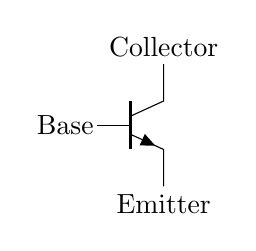
\begin{tikzpicture}
            \draw (0,0) node [npn] (transistor) {};
            \node at (0, 1) {Collector};
            \node at (-1.25, 0) {Base};
            \node at (0, -1) {Emitter};
        \end{tikzpicture}
        \caption{NPN transistor}
    \end{figure}
    A transistor will allow current flow from the collector to the emitter if the voltage at the base is sufficiently high (\(\sim \SI{0.6}{V}\)). The transistor above is an NPN transistor. We can tell this as the arrow always points from P type to N type and the collector and emitter are always the same type. The way that this transistor works internally is that there is a sandwich of P type semi conductor between two layers of N type semiconductor. The base current is connected to the P type layer. When the base current is high enough it creates more holes (lack of electrons) in the P type layer allowing electrons to flow from the emitter layer of the transistor to the collector layer and hence have a current flow. The current flow for sufficiently high base voltage is given by
    \[I_E=I_B+I_C\]
    This follows from Kirchhoff's current law as the current flow into the transistor is \(I_B+I_C\) so this must be the current that flows out as well.
    
    For sufficiently high base current it is still possible that the current flow is lower than expected as the layer of the transistor connected to the collector becomes saturated with charge carriers and the voltage isn't high enough to move them. This typically occurs for \(V_C<\SI{0.5}{V}\).
    
    If both base and collector voltages are high enough then we have the relationship:
    \begin{equation}\label{eqn:IC=betaIB}
        I_C=\beta I_B
    \end{equation}
    where \(\beta\) is a constant of proportionality.
    
    If \(I_C<\beta I_B\) then the external circuit is limiting the transistor not the base voltage.
    
    In the linear (activation) region where both base and collector voltages are sufficiently high:
    \[I_B=I_S'e^{V_{BE}/V_T}\]
    where \(I_S'\) is an unknown constant (although it actually varies a lot with temperature). \(V_{BE}\) is the potential difference across the base and emitter. \(V_T\) is given by
    \[V_T=\frac{kT}{q}\]
    where \(k = \num{1.38e-23}~\si{m^2.kg\s^{-2}.K^{-1}}\) is the Boltzmann constant, \(T\approx \SI{300}{K}\) is the temperature and \(q = \num{1.6e-19}~\si{C}\) is the charge of an electron. This gives an approximate value of \(V_T\approx \SI{25.8}{mV}\).
    Substituting this into \(I_C=\beta I_B\) and combining unknown constants we get:
    \[I_C=\beta I_s'e^{V_{BE}/V_T}=I_se^{V_{BE}/V_T}\]
    
    \section{Amplifiers}
    \subsection{Transistor Bias}
    For a transistor to remain in the active region the base voltage must have a non-zero value.
    The output must also have non-zero average values. Defining these values is called setting the DC bias.
    
    \begin{figure}[ht]
        \centering
        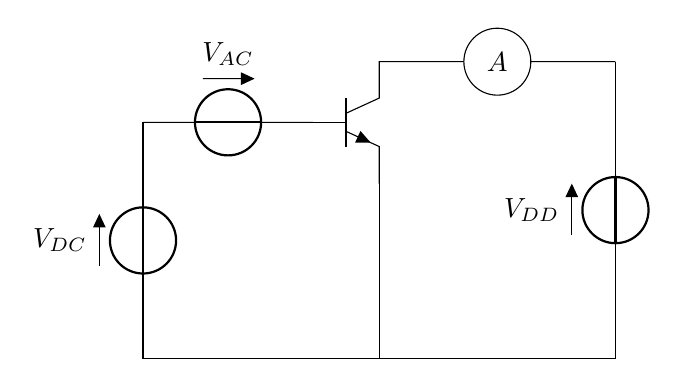
\begin{tikzpicture}
            %\draw[lightgray] (0, 0) grid (7, 5);
            \draw (0, 0) to[V=\(V_{DC}\)] (0, 3);
            \draw (3, 3) node[npn](transistor) {} (transistor.base) node[anchor=east] {};
            \draw (0, 3) to[V=\(V_{AC}\)] (transistor.base);
            \draw (transistor.collector) -- (6, 3.77);
            \draw[fill=white] (4.5, 3.77) circle (0.425cm);
            \node at (4.5, 3.77) {\(A\)};
            \draw (6, 0) to[V=\(V_{DD}\)] (6, 3.77);
            \draw (0, 0) -- (6, 0);
            \draw (3, 0) -- (transistor.emitter);
        \end{tikzpicture}
        \caption{A simple circuit to set transistor bias}
        \label{Simple transistor bias}
    \end{figure}
    Figure~\ref{Simple transistor bias} is a basic example of a circuit for setting the bias. 
    A more likely circuit for this is shown in figure~\ref{Complicated transistor bias}
    
    \begin{figure}[ht]
        \centering
        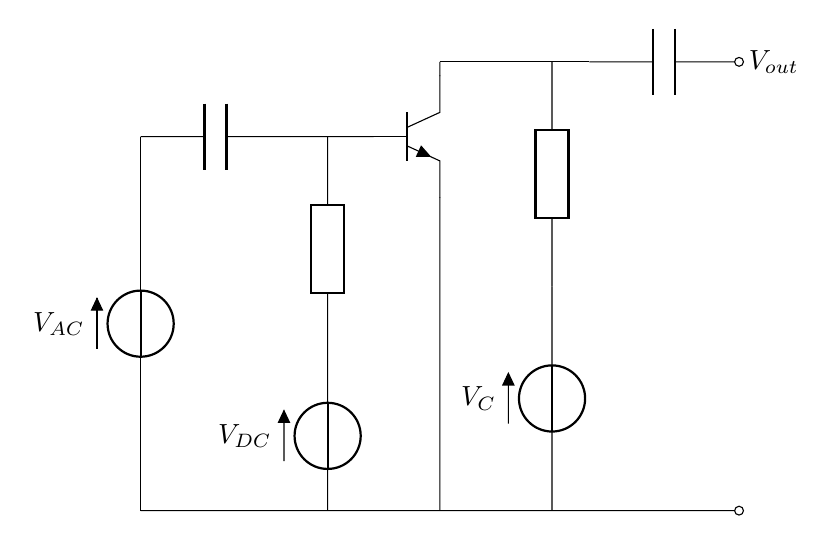
\begin{tikzpicture}[scale=0.95]
            %\draw[lightgray] (0, 0) grid (8, 8);
            \draw (4, 7) node[npn](transistor) {} (transistor.base) node[anchor=east] {};
            \draw (0, 7) to[C] (2, 7);
            \draw (2, 7) -- (transistor.base);
            \draw (2.5, 2) to[V=\(V_{DC}\)] (2.5, 4);
            \draw (2.5, 4) to[R] (2.5, 7);
            \draw (0, 2) to[V=\(V_{AC}\)] (0, 7);
            \draw (4, 2) -- (transistor.emitter);
            \draw (transistor.collector) -- (4, 8);
            \draw (4, 8) -- (6, 8);
            \draw (6, 8) to[C, -o] (8, 8);
            \node[right] at (8, 8) {\(V_{\text{out}}\)};
            \draw (5.5, 8) to[R] (5.5, 5);
            \draw (5.5, 2) to[V=\(V_{C}\)] (5.5, 5);
            \draw (0, 2) to[short, -o] (8, 2);
        \end{tikzpicture}
        \caption{A more realistic circuit to set transistor bias}
        \label{Complicated transistor bias}
    \end{figure}

    \subsection{Transistors as Amplifiers}\label{previous calculation for small signal analysis}
    An amplifier increases the amplitude of a signal. 
    In practice this means that it increases the voltage. 
    An inverting amplifier also changes the sign on the voltage so a positive input will have a negative output and the absolute size of the output is bigger than that of the input. 
    Figure~\ref{single transistor inverting amplifier} uses a transistor as an inverting amplifier. This circuit is not suitable for integration with an integrated chip as the resistor is too large. 
    This is a non-linear circuit. 
    The AC gain is given by \(\Delta V_{\text{out}}/\Delta V_{\text{in}}\). If \(V_{\text{in}}\approx \SI{0.6}{V}\)  and \(V_\text{out}\in [0, V_{C}]\) then the transistor is in the linear region.
    
    \begin{figure}[ht]
        \centering
        \begin{tikzpicture}
            %\draw[lightgray] (0, 0) grid (2, 6);
            \draw (0, 0) -- (2, 0) node[ground]{};
            \draw (1, 1) node[npn](transistor) {};
            \draw (transistor.base) to[short, -o] (0, 1);
            \node[left] at (0, 1) {\(V_{\text{in}}\)};
            \draw (transistor.emitter) -- (1, 0);
            \draw (transistor.collector) -- (1, 2);
            \draw (1, 2) to[short, -o] (2, 2);
            \node[right] at (2, 2) {\(V_{\text{out}}\)};
            \draw (1, 2) -- (1, 3);
            \draw[->] (1, 3) -- (1, 2.5);
            \node[left] at (1, 2.5) {\(I_C\)};
            \draw (1, 3) to[R=\(R\)] (1, 5);
            \draw (0, 5) -- (2, 5);
            \node[right] at (2, 5) {\(V_{DD}\)};
        \end{tikzpicture}
        \caption{A single transistor inverting amplifier}
        \label{single transistor inverting amplifier}
    \end{figure}

    One question that we need to ask is \emph{What is the optimum value for \(V_C\)?} If you turn transistor hard on you get \(V_C\approx \SI{0.2}{V}\). If you turn the transistor off you get \(V_C=\SI{5}{V}\). A good choice for \(V_C\) is halfway between these values \(V_C=(5+0.2)/2=\SI{2.6}{V}\)
    
    Another more realistic circuit introduces some resistance as in figure~\ref{amplifier with resistance}
    
    \begin{figure}[ht]
        \centering
        \begin{tikzpicture}
            %\draw[lightgray] (0, 0) grid (8, 8);
            \draw (0, 2) to[C, o-] (2, 2);
            \draw (2, 2) to[R=\(R_{B1}\)] (2, 5);
            \draw (4, 2) node[npn](transistor) {};
            \draw (2, 2) -- (transistor.base);
            \draw (transistor.emitter) -- (4, 0.5);
            \draw (transistor.collector) to[R=\(R_C\)] (4, 5);
            \draw (0, 0.5) -- (5, 0.5) node[ground]{};
            \draw (0, 5) -- (5, 5);
            \node[left] at (0, 2) {\(V_\text{in}\)};
            \node[right] at (5, 5) {\(V_{DD}\)};
            \draw (4, 2.8) to[short, -o] (5, 2.8);
            \node[right] at (5, 2.8) {\(V_C\)};
        \end{tikzpicture}
        \caption{A single transistor inverting amplifier with resistance}
        \label{amplifier with resistance}
    \end{figure}
    
    Suppose \(R_C=\SI{10}{k\ohm}\), \(\beta=390\), \(V_{BE}=\SI{0.63}{V}\), \(V_{DD}=\SI{5}{V}\) and \(V_C\) is to be optimum. What is a good value for \(R_{B1}\)?
    \[V_C=\SI{2.6}{V}\implies V_{BC}=5-2.6=\SI{2.4}{V}\]
    \[I_C=\frac{\SI{2.4}{V}}{\SI{10}{k\ohm}}=\SI{0.24}{mA}\]
    \[I_B=\frac{I_C}{\beta}=\frac{\SI{240}{\mu A}}{390}=\SI{0.615}{\mu A}\]
    \[V_B=\SI{0.63}{V}\implies V_{R_{B1}}=5-0.63=\SI{4.37}{V}\]
    \[R_{B1}=\frac{\SI{4.37}{V}}{\SI{0.615}{\mu A}}=\SI{7.11}{M\ohm}\]
    In general by using the equations \(I_C=\beta I_B\), \(V_C=V_{DD}-I_CR_C\) and \(I_B=(V_{DD}-V_{BE})\) we can derive the formula
    \[V_C=V_{DD}-\beta R_C\frac{V_{DD}-V_{BE}}{R_{B1}}\]
    This is too dependant on \(\beta\) for use in actual circuits as \(\beta\) changes with temperature and even at the correct operating temperature the actual value of \(\beta\) quoted on the transistor can be upto \SI{50}{\%} off. Adding to this the large size of \(R_{B1}\) means that this isn't a good circuit for actual use.
    
    \subsection{Gains}
    Some circuits have the same AC and DC gains but others don't. The definitions of these gain types are:
    \[
        \begin{array}{cc}
            \text{DC gain} = \frac{V_\text{out}}{V_\text{in}} & \text{AC gain} = \dv{V_\text{out}}{V_\text{in}}
        \end{array}
     \]
     From earlier we had 
     \[I_C=I_Se^{V_{BE}/V_T}\]
     so \(I_C\) varies with \(V_\text{in}=V_{BE}\). To find the AC gain \(g_m\):
     \begin{equation}\label{eqn:gm=IC/VT}
        gm = \frac{\Delta I_C}{\Delta V_{BE}}=\dv{I_C}{V_{BE}}=\frac{1}{V_T}I_Se^{V_{BE}/V_T}=\frac{I_C}{V_T}
     \end{equation}
     \section{Gain}
     
     To measure the gain \(g_m\) of any component we draw an \(I_\text{out}/V_\text{in}\) graph and differentiate to find \(g_m\).
     For a bipolar transistor this is the same as using the circuit in figure~\ref{fig:transistor gain}.
     
     \begin{figure}[ht]
         \centering
         \begin{tikzpicture}
             %\draw[lightgray] (0, 0) grid (5, 5);
             \draw (0, 0) -- (2, 0);
             \draw (1, 1) node [npn] (transistor) {};
             \draw (transistor.emitter) -- (1, 0);
             \draw (transistor.collector) -- (1, 3);
             \draw (0, 3) -- (2, 3);
             \draw[->] (1, 3) -- (1, 2.5);
             \node[right] at (1, 2.5) {\(I_C\)};
             \node[left] at (transistor.base) {\(V_{BE}\)};
             \draw (2, 0) node [ground] () {};
         \end{tikzpicture}
         \caption{Circuit for calculating the gain of a transistor}
         \label{fig:transistor gain}
     \end{figure}
    \[g_m = \frac{I_C}{V_T}\implies [g_m] = \frac{\si{A}}{\si{V}} = \si{\ohm^{-1}} = \text{Siemens} = \si{S}\]
    If we vary \(V_\text{in}\) while fixing \(V_{DD} = \SI{5}{V}\) and \(R_C = \SI{10}{k\ohm}\) and then plot the result of \(V_\text{out}\) we get the graph in figure~\ref{fig:v_in-v_out graph}
    
    \begin{figure}[ht]
        \centering
        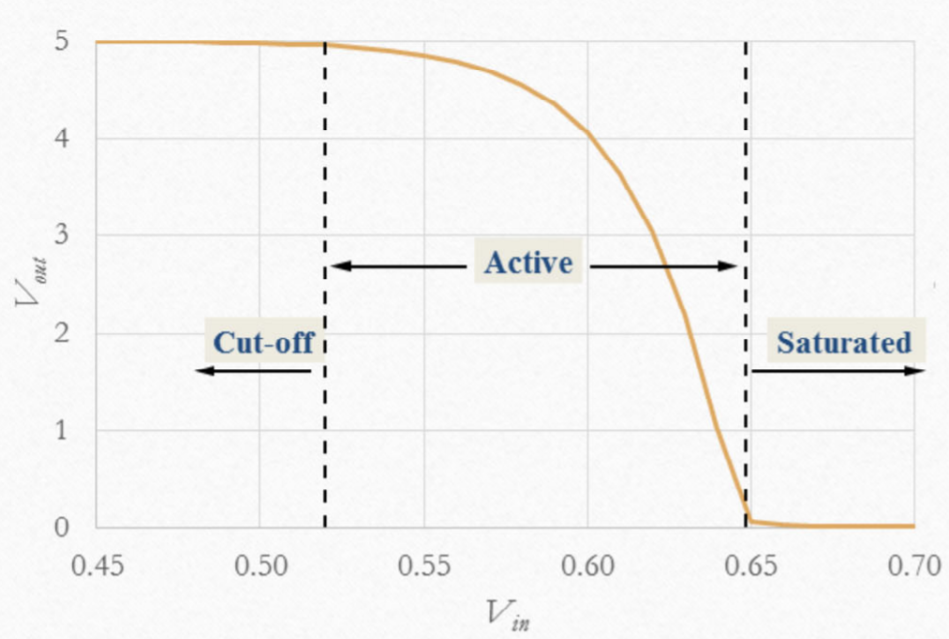
\includegraphics[scale=0.5]{v_in_vs_v_out}
        \caption{A graph of \(V_\text{in}\) vs \(V_\text{out}\) for calculating gain}
        \label{fig:v_in-v_out graph}
    \end{figure}

    The gain isn't linear but if we operate over a small enough region of input values we can approximate it as linear.
    We typically operate in the region from \SI{0.60}{V} to \SI{0.63}{V} as the steepness of the graph shows there is large gain here but we are far enough from the saturated region that we aren't accidentally going to enter it.
    
    The value of the AC gain depends on the bias conditions. We represent the AC part of a voltage or current with lower case (eg the AC component of \(V_\text{out}\) is \(v_\text{out}\). \(v_\text{out}\) depends on \(i_C\). \(i_C\) depends on \(v_\text{in}\) in a non-linear manner. More generaly for bipolar transistors \(v_\text{in} = v_\text{BE}\) therefore we care about how \(i_C\) varies with \(v_{BE}\).
    
    \subsection{Current Sink}
    A current sink permits constant current to pass. A primitive current sink can be made with a transistor as in figure~\ref{fig:primitive current sink}
    
    \begin{figure}[ht]
        \centering
        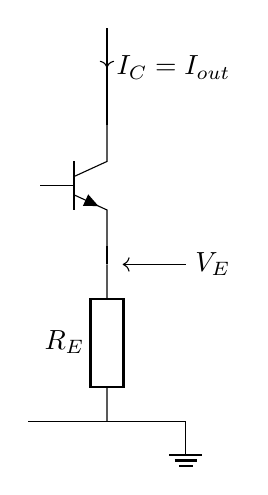
\begin{tikzpicture}
            %\draw[lightgray] (0, 0) grid (3, 5);
            \draw (0, 0) -- (2, 0) node [ground] {};
            \draw (1, 0) to[R=\(R_E\)] (1, 2);
            \draw (1, 3) node[npn](transistor) {};
            \draw (transistor.emitter) -- (1, 2);
            \draw (transistor.collector) -- (1, 5);
            \draw[->] (1, 5) -- (1, 4.5);
            \node[right] at (1, 4.5) {\(I_C=I_\text{out}\)};
            \draw[->] (2, 2) -- (1.2, 2);
            \node[right] at (2, 2) {\(V_E\)};
        \end{tikzpicture}
        \caption{A primitive current sink made with an NPN transistor}
        \label{fig:primitive current sink}
    \end{figure}

    \[V_\text{in} = V_E + 0.6 = I_ER_E + 0.6\]
    \[I_C\approx I_E\implies I_C\approx \frac{(V_\text{in} - 0.6)}{R_E}\]
    Note that \(I_C\) is independent of resistance in the collector wire.
    
    Using this with \(I_B = \SI{5}{\mu A}\) we get the graph in figure~\ref{fig:sink V_C-I_C}
    
    \begin{figure}[ht]
        \centering
        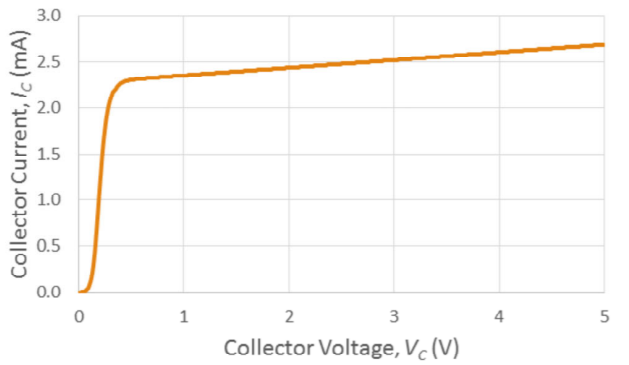
\includegraphics[scale=0.7]{v_c_vs_i_c}
        \caption{A graph of \(V_C\) against \(I_C\) for a transistor based current sink}
        \label{fig:sink V_C-I_C}
    \end{figure}
    
    A fairly effective current source can also be constructed in a similar manner using a PNP transistor as seen in figure~\ref{fig:primitive current source}.
    
    \begin{figure}[ht]
        \centering
        \begin{tikzpicture}
            %\draw[lightgray] (0, 0) grid (5, 5);
            \draw (0, 5) -- (2, 5) node[right] {\(V_{DD}\)};
            \draw (1, 5) to[R=\(R_E\)] (1, 3);
            \draw (1, 2) node[npn](transistor) {};
            \node[left] at (transistor.base) {\(V_\text{in}\)};
            \draw (transistor.collector) -- (1, 3);
            \draw (transistor.emitter) -- (1, 0);
            \draw[->] (1, 0) -- (1, 0.5) node[right] {\(I_C=I_\text{out}\)};
        \end{tikzpicture}
        \caption{A primitive current source made with a PNP transistor}
        \label{fig:primitive current source}
    \end{figure}
    
    A differential amplifier (figure~\ref{fig:differential amplifier}) instead of amplifying a current amplifies the difference between two currents. It is important that both transistors have the same value for \(\beta\). For this reason they are constructed on one piece of silicon together. We call them matched transistors.
    
    \begin{figure}[ht]
        \centering
        \begin{tikzpicture}
            \draw (0, 0) node[ground] {};
            \draw (0, 0) to[I=\(I_\text{bias}\)] (0, 2);
            \draw (-1, 2) -- (1, 2);
            \draw (-1, 3) node[npn] (transistor1) {};
            \draw (1, 3) node[npn, xscale=-1] (transistor2) {};
            \node[left] at (transistor1.base) {\(V_\text{in1}\)};
            \node[right] at (transistor2.base) {\(V_\text{in2}\)};
            \draw (transistor1.emitter) -- (-1, 2);
            \draw (transistor2.emitter) -- (1, 2);
            \draw (transistor1.collector) to[R=\(R_C\)] (-1, 6);
            \draw (transistor2.collector) to[R=\(R_C\)] (1, 6);
            \draw (-1.5, 6) -- (1.5, 6);
            \draw (-1, 4) -- (-1.5, 4) node[left] {\(V_\text{out1}\)};
            \draw (1, 4) -- (1.5, 4) node[right] {\(V_\text{out2}\)};
        \end{tikzpicture}
        \caption{A differential amplifier}
        \label{fig:differential amplifier}
    \end{figure}
    For this to work we need \(V_E>\sim \SI{0.7}{V}\) for the current sink \(I_\text{bias}\) to work and we need \(V_\text{in1}\) and \(V_\text{in2}\) to be larger than about \SI{1.3}{V}.
    
    \section{Op-Amp}
    We can define an average voltage for the inputs of \(V_\text{in}\). 
    A common occurrence is that 
    \[V_\text{in1} = V_\text{in} + \Delta V \qquad \& \qquad V_\text{in2} = V_\text{in} - \Delta V\]
    for some small \(\Delta V\) which is the analogue component of the voltage where as \(V_\text{in}\) is the digital component.
    From this we get 
    \[I_{C1} = I_\text{bias}/2 + g_m\Delta V \qquad \& \qquad I_{C2} = I_\text{bias}/2 - g_m\Delta V\]
    \[V_\text{out1} = V_{DD} - I_{C1}R_C = V_{DD} - R_C(I_\text{bias}/2 + g_m\Delta V)\]
    \[V_\text{out2} = V_{DD} - R_C(I_\text{bias}/2 - g_m\Delta V)\]
    If we take our output as the difference between the outputs
    \[V_\text{out1} - V_\text{out2} = V_{DD} - R_C(I_\text{bias}/2 + g_m\Delta V) - V_{DD} + R_C(I_\text{bias}/2 - g_m\Delta V) = -2R_Cg_m\Delta V\]
    If we then use the fact that \(V_\text{in1} - V_\text{in2} = 2\Delta V\) we can calculate gain
    \[\text{gain} = \frac{\text{output}}{\text{input}} = -\frac{R_Cg_m\Delta V}{2\Delta V} = -R_Cg_m\]
    \[g_m = \frac{I_C}{V_T} = \frac{I_\text{bias}/2}{V_T} = \frac{I_\text{bias}}{2V_T}\]
    \[\text{gain} = -\frac{R_CI_\text{bias}}{2V_T}\]
    \[\text{gain} \propto I_\text{bias}\]
    We can use this to make a variable gain amplifier. 
    We actually need the difference \(V_\text{out1} - V_\text{out2}\) so we need a single-ended output differencing circuit.
    For this we use an op-amp as in figure~\ref{fig:op-amp differencing circuit}.\label{text reference differencing circuit}
    
    \subsection{The Op-amp}
    To avoid working with individual semiconductor components we use integrated circuits (IC) which are:
    \begin{itemize}
        \item guaranteed to work
        \item cheap
        \item light
        \item robust
        \item low power
    \end{itemize}
    The simplest IC is an operational amplifier or op-amp with the circuit diagram shown in figure~\ref{fig:op-amp}. 
    It is a three terminal device (excluding power supplies). 
    It is actually an IC full of transistors, resistors and capacitors.
    Its sole function is to make its output proportional to the difference between its inputs.
    \[V_\text{out} = A(V_+-V_-)\]
    where \(A\) is a large (\(\sim10^5\)) amplifying factor that depends on the individual op-amp.
    \begin{figure}[ht]
        \centering
        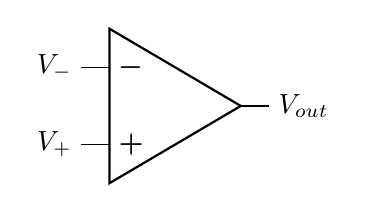
\begin{tikzpicture}% table
            \node[op amp] (op-amp) at (0, 0) {};
            \node[left] at (op-amp.-) {\(V_-\)};
            \node[left] at (op-amp.+) {\(V_+\)};
            \node[right] at (op-amp.out) {\(V_\text{out}\)};
        \end{tikzpicture}
        \caption{Op-amp circuit diagram}
        \label{fig:op-amp}
    \end{figure}

    No current goes into the terminals of an op amp.
    Its output can supply any current required.
    The previous two statements are approximations. 
    A good op-amp will have \(I_\text{in}\approx\num{10e-12}\) and \(R_\text{out} \approx \SI{100}{\ohm}\) which means it will lose some current at output.
    
    An op-amp needs power supplies as shown in figure~\ref{fig:powered op-amp}. 
    They are almost never shown on a circuit diagram.
    The output of the op-amp can't exceed the power supply's, usually it is less. 
    The inputs usually shouldn't go outside of the power supply range.
    
    \begin{figure}[ht]
        \centering
        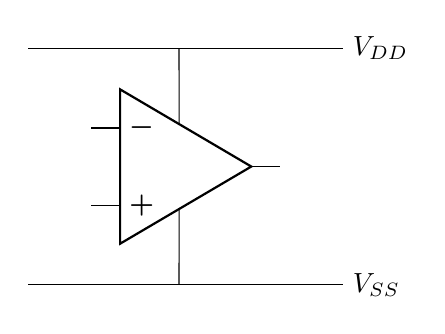
\begin{tikzpicture}
            %\draw[lightgray] (-3, -3) grid (3, 3);
            \node[op amp] (op-amp) at (0, 0) {};
            \draw (op-amp.up) -- (-0.085, 1.5);
            \draw (op-amp.down) -- (-0.085, -1.5);
            \draw (-2, 1.5) -- (2, 1.5) node[right] {\(V_{DD}\)};
            \draw (-2, -1.5) -- (2, -1.5) node[right] {\(V_{SS}\)};
        \end{tikzpicture}
        \caption{A powered op-amp}
        \label{fig:powered op-amp}
    \end{figure}
    
    Assume \(A=\num{e5}\), use \(\SI{\pm 15}{V}\) power supplies, make \(V_+=\SI{12}{V}\) and \(V_-=\SI{-12}{V}\).
    \[V_\text{out} = 10^5(12-(-12))=\SI{2.4}{MV}\]
    This is unlikely, in reality \(V_\text{out}\) will saturate at an upper limit, or if instead \(V_+\) is negative and \(V_-\) is positive it will saturate at some lower input. \(V_\text{out}=A(V_+-V_-)\) is only true if \(V_\text{out}\) is not saturated.
    
    Lets assume \(V_\text{out}\) isn't saturated.
    \[V_\text{out} = A(V_+-V_-)\]
    \[V_+-V_-=\frac{V_\text{out}}{A}\]
    \(V_\text{out}\) is small and \(A\) is large so \(V_+-V_-\) is very small so \(V_+\approx V_-\).
    
    \subsection{Golden Rules}
    The golden rules of op-amps are:
    \begin{itemize}
        \item No current flows into the inputs
        \item An op-amp can supply any current
        \item \(V_+=V_-\) if \(V_\text{out}\) is not saturated
    \end{itemize}

    We can make an inverting op-amp amplifier using the circuit in figure~\ref{fig:op-amp inverting amplifier}. 
    We assume positive and negative power supplies. 
    \(V_+\) is grounded so \(V_+=0\), from the golden rules we know \(V_-=0\).
    The connection from \(V_\text{out}\) to \(V_-\) keeps \(V_+=V_-\)
    
    \begin{figure}[ht]
        \centering
        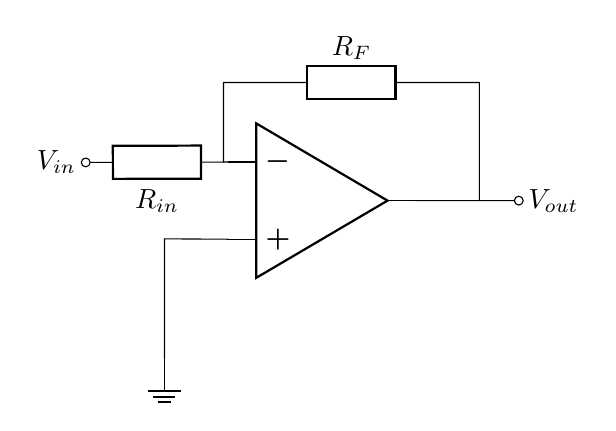
\begin{tikzpicture}
            %\draw[lightgray] (0, 0) grid (6, 6);
            \node[op amp] (opamp) at (3, 3) {};
            \draw (opamp.-) to[R=\(R_\text{in}\), -o] (0, 3.485) node[left] {\(V_\text{in}\)};
            \draw (opamp.+) -- (1, 2.5145) -- (1, 1) node[ground] {};
            \draw (1.75, 3.485) -- (1.75, 4.5) to[R=\(R_F\)] (5, 4.5) -- (5, 3);
            \draw (opamp.out) to[short, -o] (5.5, 3) node[right] {\(V_\text{out}\)};
        \end{tikzpicture}
        \caption{An inverting op-amp amplifier}
        \label{fig:op-amp inverting amplifier}
    \end{figure}
    \[\frac{V_\text{in}-0}{R_\text{in}} + \frac{V_\text{out}-0}{R_F}=0\]
    \[\frac{V_\text{out}}{V_\text{in}} = -\frac{R_F}{R_\text{in}}=\text{gain}\]
    In this circuit gain depends on resistor ratio not on the parameters of the op-amp.
    
    We can use the modified circuit in figure~\ref{fig:op-amp differencing circuit} as the differencing circuit mentioned in section~\ref{text reference differencing circuit}
    
    \begin{figure}[ht]
        \centering
        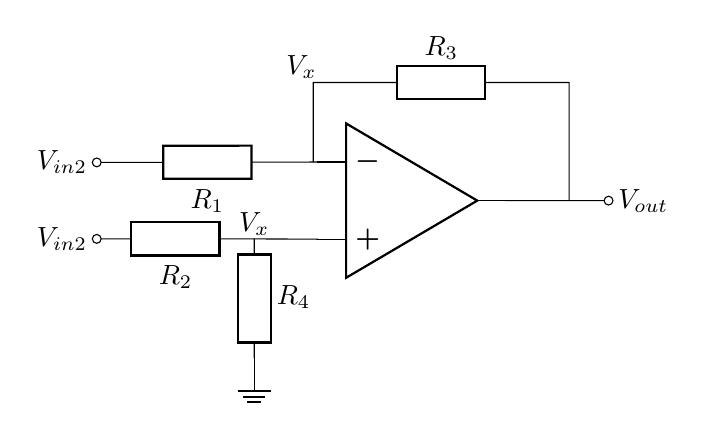
\begin{tikzpicture}
            %\draw[lightgray] (0, 0) grid (6, 6);
            \node[op amp] (opamp) at (3, 3) {};
            \draw (opamp.-) to[R=\(R_1\), -o] (-1, 3.485) node[left] {\(V_\text{in2}\)};
            \draw (opamp.+) -- (1, 2.514) to[R=\(R_4\)] (1, 1) node[ground] {};
            \draw (1.75, 3.485) -- (1.75, 4.5) to[R=\(R_3\)] (5, 4.5) -- (5, 3);
            \draw (opamp.out) to[short, -o] (5.5, 3) node[right] {\(V_\text{out}\)};
            \draw (1, 2.514) to[R=\(R_2\), -o] (-1, 2.514) node[left] {\(V_\text{in2}\)};
            \node at (1.6, 4.7) {\(V_x\)};
            \node at (1, 2.7) {\(V_x\)};
        \end{tikzpicture}
        \caption{Op-amp differencing circuit}
        \label{fig:op-amp differencing circuit}
    \end{figure}
    
    \[\frac{V_\text{in1}-V_x}{R_1} + \frac{V_\text{out}-V_x}{R_3} = 0\]
    \[\frac{V_\text{in2}-V_x}{R_2} + \frac{0 - V_x}{R_4} = 0\]
    \[\implies V_x = V_\text{in2}\frac{R_4}{R_2 + R_4}\]
    From this we can derive the result
    \[V_\text{out}=V_\text{in2}\frac{R_4(R_1+R_3)}{R_1(R_2+R_4)} - V_\text{in}\frac{R_3}{R_1}\]
    This is difficult to analyse so we use \(R_2=R_1\) and \(R_4=R_3\) to simplify. This gives us
    \[V_\text{out} = \frac{R_3}{R_1}(V_\text{in2} - V_\text{in1})\]
    
    \begin{example}
        Let \(V_\text{in1} = 3 + \sin(2\pi ft)\), \(V_\text{in2} = 3 - \sin(2\pi ft)\),  \(R_1=R_2=\SI{1}{k\ohm}\) and \(R_3=R_4=\SI{3.9}{k\ohm}\). 
        Assuming that the amplifier doesn't saturate find \(V_\text{out}\). 
        What would be a reasonable supply voltage?
        \begin{align*}
            V_\text{out} &= \frac{\SI{3.9}{k\ohm}}{\SI{1}{k\ohm}}(3 - \sin(2\pi ft) - 3 - \sin(2\pi ft))\\
            &= 3.9(-2\sin(2\pi ft))\\
            &= -7.8\sin(2\pi ft)
        \end{align*}
        \(|V_\text{out}|\) is at most \SI{7.8}{V} so a power supply of \SI{9}{V} would be reasonable.
    \end{example}

    In practice a power supply of \(\pm V_{DD}\) isn't practical so we use a single sided power supply with \(V_{DD}\) and \SI{0}{V}. 
    This gives us a reference voltage of \(V_DD/2\) instead of \SI{0}{V}.
    \[\frac{V_\text{in2}-V_x}{R_2} + \frac{V_{DD}/2 - V_x}{R_4} = 0\]
    \[\implies V_x = V_\text{in2}\frac{R_4 + R_2V_{DD}/2}{R_2+R_4}\]
    \[\implies V_\text{out} = \frac{R_3}{R_1}(V_\text{in2}-V_\text{in1}) + \frac{V_{DD}}{2}\]
    
    We can use the equivalent circuit in figure~\ref{fig:equivalent circuit} to produce a voltage source of \SI{2.5}{V} and impedance of \(R_4\). 
    
    \begin{figure}[ht]
        \centering
        \begin{tikzpicture}
            %\draw[lightgray] (0, 0) grid (3, 3);
            \draw (3, 0) to[short, o-] (0, 0) to[V=\SI{2.5}{V}] (0, 3) to[R=\(R_4\), -o] (3, 3);
        \end{tikzpicture}
        \caption{Equivalent circuit for inverting op-amp amplifier}
        \label{fig:equivalent circuit}
    \end{figure}

    The circuit in figure~\ref{fig:equivalent circuit} is difficult as \SI{2.5}{V} sources are hard to come by so instead we use the circuit in~\ref{fig:potential divider} with both resistors set to \(2R_4\) and a voltage of \SI{5}{V} which is much more common for a voltage source
    
    In a differential amplifier like in figure~\ref{fig:differential amplifier} both transistors act as variable current sources as they are in the active region. This means we can model both outputs as in figure~\ref{fig:current source differential amplifier}
    
    \begin{figure}[ht]
        \centering
        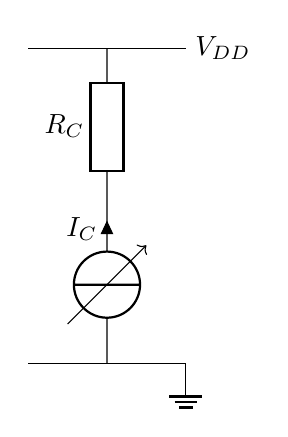
\begin{tikzpicture}
            \draw (0, 0) -- (2, 0) node [ground] {};
            \draw (1, 0) to[I=\(I_C\)] (1, 2) to[R=\(R_C\)] (1, 4);
            \draw (0, 4) -- (2, 4) node[right] {\(V_{DD}\)};
            \draw[->] (0.5, 0.5) -- (1.5, 1.5);
        \end{tikzpicture}
        \caption{Current source model of half a differential amplifier}
        \label{fig:current source differential amplifier}
    \end{figure}

    This can in turn be replaced with a Thevenin equivalent circuit such as in figure~\ref{fig:equivalent circuit to half differential amplifier}.
    
    \begin{figure}[ht]
        \centering
        \begin{tikzpicture}
            \draw node [ground] (0, 0) {} to[battery1=\(V_{DD}-I_CR_C\)] (0, 2) to[R=\(R_C\), -o] (2, 2);
        \end{tikzpicture}
        \caption{Thevenin equivalent circuit for half of a differential amplifier}
        \label{fig:equivalent circuit to half differential amplifier}
    \end{figure}
    
    This and our transistorised differential stage could be connected straight to the op-amp. 
    Since \(R_1=R_2\) we can use \(R_1\) as \(R_C\) saving on resistors when we combine the two circuits as in figure~\ref{fig:op-amp differential amplifier}.
    
    \begin{figure}[ht]
        \centering
        \begin{tikzpicture}
            %\draw[lightgray] (-3, 0) grid (9, 8);
            \draw (0, 0) node[ground] {};
            \draw (0, 0) to[I=\(I_\text{bias}\)] (0, 2);
            \draw (-1, 2) -- (1, 2);
            \draw (-1, 3) node[npn] (transistor1) {};
            \draw (1, 3) node[npn, xscale=-1] (transistor2) {};
            \node[left] at (transistor1.base) {\(V_\text{in1}\)};
            \node[right] at (transistor2.base) {\(V_\text{in2}\)};
            \draw (transistor1.emitter) -- (-1, 2);
            \draw (transistor2.emitter) -- (1, 2);
            \draw (transistor1.collector) to[R=\(R_C\)] (-1, 6);
            \draw (transistor2.collector) to[R=\(R_C\)] (1, 6);
            \draw (-1.5, 6) -- (1.5, 6) node[right] {\(V_{DD}\)};
            \draw (-1, 4) -- (-2.2, 4);
            \draw (1, 4) -- (1.5, 4);
            \begin{scope}[xshift=1cm]
                \node[op amp] (opamp) at (5, 3) {};
                \draw (-3.2, 4) -- (-3.2, 7) -- (3, 7) -- (3, 3.485) -- (opamp.-);
                \draw (2.5, 0) -- (3.5, 0) node[right] {\SI{2.5}{V}};
                \draw (3, 0) to[R=\(R_A\)] (3, 2.5145) -- (opamp.+);
                \draw (opamp.out) to[short, -o] (6.5, 3) node[right] {\(V_\text{out}\)};
                \draw (6.2, 3) -- (6.2, 5) to[R=\(R_A\)] (3, 5);
            \end{scope}
            \draw (1.5, 4) -- (3, 4) -- (3, 2.5145) -- (4, 2.5145);
        \end{tikzpicture}
        \caption{Differential amplifier and op-amp connected to make one amplifier}
        \label{fig:op-amp differential amplifier}
    \end{figure}

    \section{Transistor Models}
    \subsection{Linearity and Superposition}
    A linear system \(F\) has the property that
    \[F(a + b) = F(a) + F(b)\]
    If a system is linear then we can apply the superposition technique to analyse it.
    Transistors and diodes aren't linear, since \(I_c = I_se^{V_{BE}/V_T}\), however, it is possible to approximate them as linear as long as a reasonable DC bias is applied and \(V_{BE}\) doesn't vary too much. 
    This means that we can use superposition to separate AC and DC signals.
    
    \example
    \begin{figure}[ht]
        \centering
        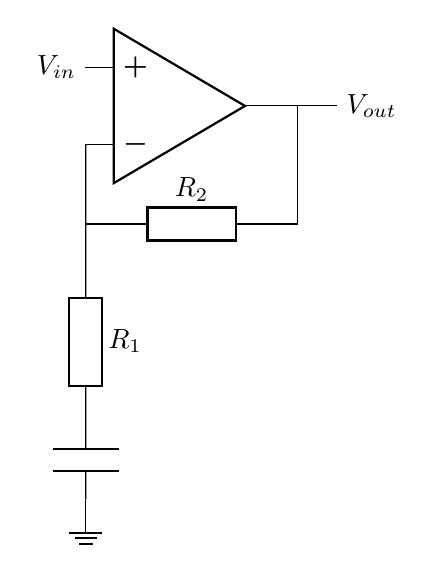
\begin{tikzpicture}
            %\draw[lightgray] (0, 0) grid (5, 5);
            \draw node[op amp, yscale=-1](opamp) at (2, 5) {};
            \draw (opamp.-) -- (0.81, 3) to[R=\(R_1\)] (0.81, 1) to[C] (0.81, 0) node[ground] at (0.81, 0) {};
            \draw (0.81, 3.5) to[R=\(R_2\)] (3.5, 3.5) -- (3.5, 5);
            \draw (opamp.out) -- (4, 5) node[right] at (4, 5) {\(V_\text{out}\)};
            \node[left] at (opamp.+) {\(V_\text{in}\)};
        \end{tikzpicture}
        \caption{Circuit for superposition analysis}
        \label{fig:superposition circuit}
    \end{figure}
    
    We can analyse the circuit in figure \ref{fig:superposition circuit} using superposition.
    If \(V_\text{in}(t) = 2.5 + A\sin(2\pi ft)\) what is \(V_\text{out}(t)\)?
    
    First determine the response with \(V_\text{in}(t) = 2.5\) then with \(V_\text{in}(t) = A\sin(2\pi ft)\) then sum the outputs.
    
    For \(V_\text{in}(t) = 2.5\) we have:
    \[V_\text{in} = V_+ \approx V_-=V_\text{out} = 2.5\]
    For \(V_\text{in}(t) = A\sin(2\pi ft)\) we have:
    \[V_\text{out}(t) = \frac{R_1 + R_2}{R_1}A\sin(2\pi ft)\]
    So for \(V_\text{in}(t) = 2.5 + A\sin(2\pi ft)\) we have:
    \[V_\text{out}(t) = 2.5 + \frac{R_1 + R_2}{R_1}A\sin(2\pi ft)\]
    
    \subsection{Ebers-Moll equations}
    The Ebers-Moll equations are models that give the current at the collector of a transistor. So far we have encountered one:
    \[I_C=I_Se^{V_{BE}/V_T}\]
    This works well in the linear region of the transistor but when \(V_{BE} = 0\) we get \(I_C=I_S\) which is wrong. 
    It should be \(I_C=0\). To fix this we use a modified version of the equation:
    \[I_C=I_S\left(e^{V_{BE}/V_T}-1\right)\]
    The \(-1\) means that at \(V_{BE}=0\) we get the correct value of \(I_C=0\).
    This makes this a good model for low \(V_{BE}\).
    At normal operating values of \(V_{BE}\) however \(e^{V_{BE}/V_T} \gg 1\) so we can ignore the \(-1\) and we get the original equation back.
    
    Another modification can be made to account for the early effect (page \pageref{early effect} section \ref{early effect}). This equation is
    \[I_C = I_Se^{V_{BE}/V_T}\left(1 - \frac{V_{CE}}{V_A}\right)\]
    where \(V_A\) is the early effect voltage (negative for an NPN transistor).
    Most of the time the unmodified version is sufficient when operating a transistor in the linear region.
    
    \subsection{Transistor Model}
    A bipolar transistor is not linear. We can, however, replace it with a linear model. 
    We use a small signal (only works for AC analysis with small voltages \((\sim \SI{0.5}{V})\)) model. 
    The common one for a transistor is shown in figure \ref{fig:transistor model}
    
    \begin{figure}[ht]
        \centering
        \begin{tikzpicture}
            %\draw[lightgray] (0, 0) grid (10, 6);
            \node[npn](transistor) at (0, 3) {};
            \node[left] at (transistor.base) {\(B\)};
            \node[below] at (transistor.emitter) {\(E\)};
            \node[above] at (transistor.collector) {\(C\)};
            
            \draw[->] (1, 3) -- (2, 3);
            
            \draw (4, 4) to[short, -o] (3, 4) node[left] at (3, 4) {\(B\)};
            \draw (4, 4) to[R=\(r_\pi\)] (4, 2);
            \draw (4, 2) -- (6, 2);
            \draw (6, 4) to[I=\(g_mV_{BE}\)] (6, 2);
            \draw (5, 2) to[short, -o] (5, 1) node[below] at (5, 1) {\(E\)};
            \draw (6, 4) to[short, -o] (9, 4) node[right] at (9, 4) {\(C\)};
            \draw (8, 4) to[R=\(r_0\)] (8, 2) -- (6, 2);
        \end{tikzpicture}
        \caption{Transistor small signal model}
        \label{fig:transistor model}
    \end{figure}
    
    The collector current comes mostly from the dependent current source with value \(g_mV_{BE}\).
    
    From equations \ref{eqn:IC=betaIB} and \ref{eqn:gm=IC/VT} we have
    \[I_C=\beta I_B\implies I_B = \frac{I_C}{\beta}\implies\frac{1}{I_B}=\frac{\beta}{I_C}\]
    \[g_m = \dv{I_C}{V_{BE}} = \frac{I_C}{V_T}\]
    We can use this to calculate \(r_\pi\) which models the input resistance
    \begin{align*}
        r_\pi &= \frac{\Delta V_{BE}}{\Delta I_B}\\
        &= \beta\frac{\Delta V_{BE}}{\Delta I_C}\\
        &= \beta\left[\frac{\Delta I_C}{\Delta V_{BE}}\right]^{-1}\\
        &= \beta\left[\dv{I_C}{V_{BE}}\right]^{-1}\\
        &= \frac{\beta}{g_m}
    \end{align*}
    
    \subsection{Early Effect}\label{early effect}
    The early effect is that when plotted on a graph of \(V_{CE}\) against \(I_C\) all the linear sections of the transistor can be traced back to cross the \(x\) axis at the same point \(V_A\) as in figure \ref{fig:early effect}
    \begin{figure}[ht]
        \centering
        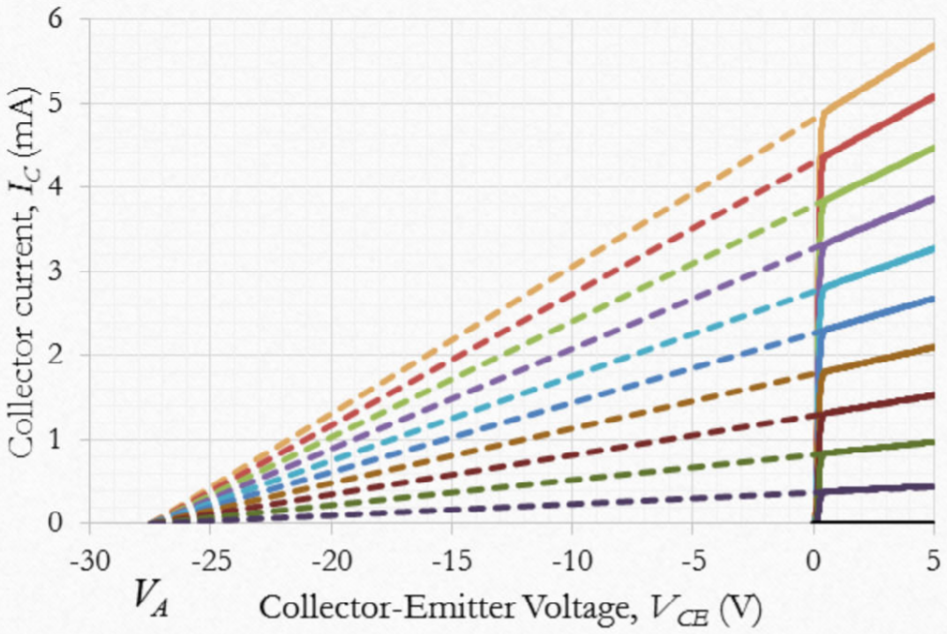
\includegraphics[scale=0.6]{early_effect.png}
        \caption{The early effect}
        \label{fig:early effect}
    \end{figure}
    The output resistance is 
    \[\dv{I_C}{V_{CE}}\]
    \(I_C\) varies with \(V_{CE}\) even in the linear region. A measure of this is the Early voltage \(V_A\). For an NPN transistor \(V_A<0\). For a PNP transistor \(V_A>0\). The larger \(|V_A|\) is the closer the linear region is to horizontal. This is desirable.
    
    The output resistance is modelled by \(r_0\) and can be calculated as
    \begin{align*}
        r_0 &= \dv{V_{CE}}{I_C}\\
        &= \left[\dv{I_C}{V_{CE}}\right]^{-1}\\
        &= \left[\dv{V_{CE}}\left(I_Se^{-V_{BE}/V_T}\left(1-\frac{V_{CE}}{V_A}\right)\right)\right]^{-1}\\
        &= \left[-\frac{I_Se^{-V_{BE}}}{V_A}\right]^{-1}\\
        &= \left[-\frac{I_C}{V_A}\right]^{-1}\\
        &= -\frac{V_A}{I_C}
    \end{align*}
    
    Small signal models are only used for AC signals (and only for small voltages). The method is:
    \begin{itemize}
        \item First assume DC biasing is correct
        \item Since we only care about AC set DC voltages to 0
        \item Decoupling (large) capacitors become short circuits
        \item Substitute the small signal model for any transistors
        \item Analyse as usual using Ohm's law, Kirchhoff's laws and other techniques
    \end{itemize}

    \example
    We can analyse the circuit in fig \ref{fig:original circuit} using this technique. 
    Figure \ref{fig:remove dc} shows the circuit after all DC voltage is set to 0 and capacitors are removed. 
    In figure \ref{fig:redrawn} the circuit is redrawn to combine the grounds and make it easier to do the final step, 
    which is shown in figure \ref{fig:final circuit} where the transistor is replaced with the small signal model.
    
    Using the values calculated on page \pageref{previous calculation for small signal analysis} section \ref{previous calculation for small signal analysis} (which are \(R_{B1} = \SI{7.11}{M\ohm}\), \(R_C = \SI{10}{k\ohm}\), \(\beta = 390\) and \(I_C = \SI{0.24}{mA}\)) we can calculate \(r_\pi\) and \(r_0\)
    \[r_\pi = \frac{\beta}{g_m} = \frac{\beta}{I_C/V_T} = \frac{\beta V_T}{I_C} = \frac{390\cdot\SI{25.3}{mV}}{\SI{0.24}{mA}}\]
    The input resistance is the total resistance due to \(R_{B1}\) and \(r_\pi\):
    \[R_{B1}\parallel r_\pi = \frac{1}{\frac{1}{R_{B1}} + \frac{1}{r_\pi}} = \SI{40.9}{k\ohm}\]
    \[r_0=-\frac{V_A}{I_C}\]
    For the BC109 transistor (which is the one we are using) \(V_A = \SI{-28.14}{V}\) (this is actually a relatively small value of \(|V_A|\)). This means that \(r_0 = \SI{28.14}{V}/\SI{0.24}{mA} = \SI{117}{k\ohm}\). The total output resistance is
    \[r_0\parallel R_C = \frac{1}{\frac{1}{r_0} + \frac{1}{R_C}} = \SI{9.21}{k\ohm}\]
    
    \begin{figure}[ht]
        \centering
        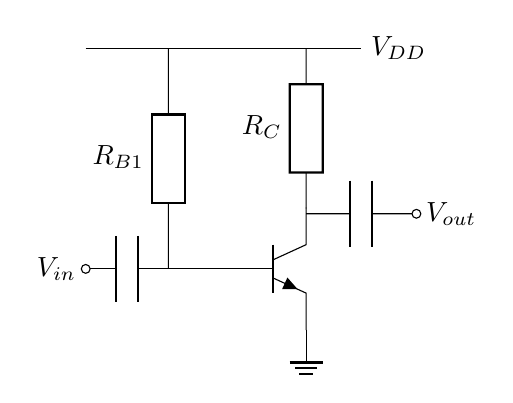
\begin{tikzpicture}[scale=0.7]
            %\draw[lightgray] (0, 0) grid (7, 5);
            \draw (0, 0) to[C, o-] (1.5, 0);
            \node[left] at (0, 0) {\(V_\text{in}\)};
            \node[npn](transistor) at (4, 0) {};
            \node[ground] at (transistor.emitter) {};
            \draw (1.5, 0) to[R=\(R_{B1}\)] (1.5, 4);
            \draw (transistor.collector) to[R=\(R_C\)] (4, 4);
            \draw (1.5, 0) -- (transistor.base);
            \draw (0, 4) -- (5, 4) node[right] at (5, 4) {\(V_{DD}\)};
            \draw (4, 1) to[C, -o] (6, 1) node[right] at (6, 1) {\(V_\text{out}\)};
        \end{tikzpicture}
        \caption{Circuit to analyse using small signal models}
        \label{fig:original circuit}
    \end{figure}

    \begin{figure}[ht]
        \centering
        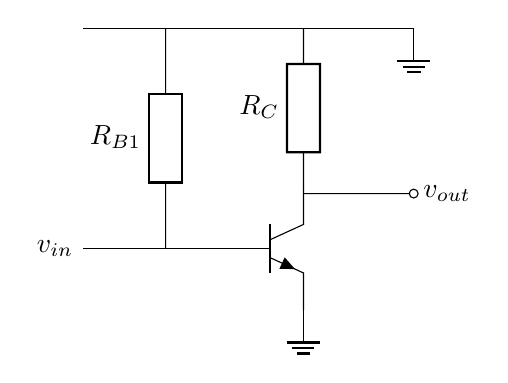
\begin{tikzpicture}[scale=0.7]
        %\draw[lightgray] (0, 0) grid (7, 5);
        \draw (0, 0) -- (1.5, 0);
        \node[left] at (0, 0) {\(v_\text{in}\)};
        \node[npn](transistor) at (4, 0) {};
        \node[ground] at (transistor.emitter) {};
        \draw (1.5, 0) to[R=\(R_{B1}\)] (1.5, 4);
        \draw (transistor.collector) to[R=\(R_C\)] (4, 4);
        \draw (1.5, 0) -- (transistor.base);
        \draw (0, 4) -- (6, 4) node[ground] at (6, 4) {};
        \draw (4, 1) to[short, -o] (6, 1) node[right] at (6, 1) {\(v_\text{out}\)};
        \end{tikzpicture}
        \caption{Circuit with capacitors removed and DC bias set to 0}
        \label{fig:remove dc}
    \end{figure}

    \begin{figure}[ht]
        \centering
        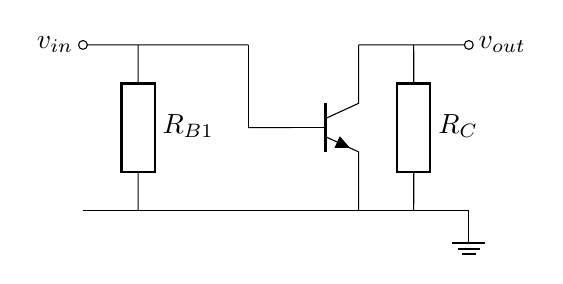
\begin{tikzpicture}[scale=0.7]
        %\draw[lightgray] (0, 0) grid (7, 5);
        \draw (0, 3) to[short, o-] (3, 3) node[left] at (0, 3) {\(v_\text{in}\)};
        \draw (0, 0) -- (7, 0);
        \draw (1, 3) to[R=\(R_{B1}\)] (1, 0);
        \draw (3, 3) -- (3, 1.5);
        \node[npn](transistor) at (5, 1.5) {};
        \draw (3, 1.5) -- (transistor.base);
        \draw (transistor.emitter) -- (5, 0);
        \draw (transistor.collector) -- (5, 3);
        \draw (5, 3) to[short, -o] (7, 3) node[right] at (7, 3) {\(v_\text{out}\)};
        \draw (6, 3) to[R=\(R_C\)] (6, 0);
        \node[ground] at (7, 0) {};
        \end{tikzpicture}
        \caption{Circuit redrawn to make later steps easier}
        \label{fig:redrawn}
    \end{figure}

    \begin{figure}[ht]
        \centering
        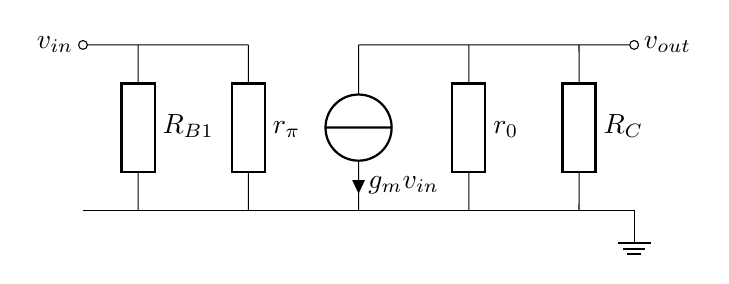
\begin{tikzpicture}[scale=0.7]
        %\draw[lightgray] (0, 0) grid (10, 5);
        \draw (0, 3) to[short, o-] (3, 3) node[left] at (0, 3) {\(v_\text{in}\)};
        \draw (0, 0) -- (10, 0);
        \draw (1, 3) to[R=\(R_{B1}\)] (1, 0);
        \draw (3, 3) to[R=\(r_\pi\)] (3, 0);
        \draw (5, 3) to[I=\(g_mv_\text{in}\)] (5, 0);
        \draw (7, 3) to[R=\(r_0\)] (7, 0);
        \draw (9, 3) to[R=\(R_C\)] (9, 0);
        \draw (5, 3) to[short, -o] (10, 3) node[right] at (10, 3) {\(v_\text{out}\)};
        \node[ground] at (10, 0) {};
        \end{tikzpicture}
        \caption{Circuit with transistor replaced}
        \label{fig:final circuit}
    \end{figure}

    \section{More Transistor Modelling}
    \[g_mv_\text{in} + \frac{v_\text{out}}{r_0} + \frac{v_\text{out}}{R_C} = 0\]
    \[\frac{v_\text{out}}{v_\text{in}} = -\frac{g_m}{\frac{1}{r_0} + \frac{1}{R_C}} = -\frac{g_m}{g_0 + G_C}\]
    where \(g_0 = 1/r_0\) and \(G_C = 1/R_C\).
    The only current in the model comes from the current source. 
    This is because \(v_\text{in}\) is AC so averages at \SI{0}{V} so \(R_{B1}\) and \(r_\pi\) are connected to \SI{0}{V} at both ends.
    The current must go through the parallel \(R_C\) and \(r_0\).
    
    If \(R_{B1}\) and \(r_\pi\) have no influence on the current source or \(r_0\) then why do we include them in the model? 
    Because they are important if we chain together multiple transistors and in determining the cut off frequency and size of the capacitor.
    
    We can increase gain by increasing \(R_C\), which decreases \(G_C\). What limits the size of \(R_C\)?
    \(R_C\) is set by the original conditions of \(I_\text{bias}\), \(V_C\) etc.
    
    The input capacitor \(C_\text{in}\) forms high pass filter. 
    That is a filter that only allows frequencies above some cut off frequency \(f_C\) to pass.
    The cut off frequency is given by
    \[f_C = \frac{1}{2\pi RC}\]
    where \(R\) is the impedance, in this case \(R = R_{B1}\parallel r_\pi\) and \(C\) is the capacitance of the capacitor.
    \[f_C = \frac{R_{B1} + r_\pi}{2\pi R_{B1} r_\pi C}\]
    Since \(R_{B1}\gg r\pi\) \((R_{B1} \approx \SI{e6}{\ohm},\,r_\pi\approx \SI{e3}{\ohm})\) we can approximate \(R_{B1} + r_\pi\approx R_{B1}\)
    \[f_C \approx \frac{R_{B1}}{2\pi R_{B1}r_\pi C} = \frac{1}{2\pi r_\pi C}\]
    
    The lowest audible frequency is about \SI{50}{Hz}. 
    We might choose a value of \SI{20}{Hz} as our cut off frequency then. 
    We can work out the capacitance required given that all other values are set by other requirements
    \[C\approx \frac{1}{2\pi r_\pi f_C} = \frac{1}{2\pi \cdot \SI{41.1}{k\ohm}\cdot\SI{20}{Hz}} = \SI{0.2}{\micro F}\]
    Note that capacitors have a layer of oxide on their anode and if connected the wrong way round this layer decomposes allowing more current through which causes the capacitor to heat up and explode.
    
    \section{Improving Linearity}
    We can use negative feedback as shown in figure \ref{fig:negative feedback} to use the external circuit to control gain instead of the transistor. 
    This improves linearity.
    \begin{figure}[ht]
        \centering
        \begin{tikzpicture}
            %\draw[lightgray] (0, 0) grid (5, 8);
            \node[npn](transistor) at (3, 3) {};
            \draw (0, 3) to[C, o-] (transistor.base);
            \node[left] at (0, 3) {\(V_\text{in}\)};
            \draw (transistor.emitter) to[R=\(R_E\)] (3, 0.5) node[ground] at (3, 0.5) {};
            \draw (3, 6) to[R=\(R_C\)] (transistor.collector);
            \draw (3, 4) to[C, -o] (5, 4) node[right] at (5, 4) {\(V_\text{out}\)};
            \draw (0, 6) -- (5, 6) node[right] at (5, 6) {\(V_{DD}\)};
            \draw (2, 3) -- (2, 3.8) to[R=\(R_{B1}\)] (2, 6);
        \end{tikzpicture}
        \caption{Negative feedback}
        \label{fig:negative feedback}
    \end{figure}
    The resistor \(R_E\) limits the change in \(I_B\) which limits the \(I_C\).
    We can use the small signal model as in figure \ref{fig:negative feedback small signal} to do some more analysis.
    \begin{figure}[ht]
        \centering
        \begin{tikzpicture}
            %\draw[lightgray] (0, 0) grid (10, 4);
            \draw (1, 4) to[R=\(R_{B1}\)] (1, 0);
            \draw (2.5, 4) to[R=\(r_\pi\)] (2.5, 2);
            \draw (4, 4) to[I=\(g_m(v_\text{in} - v_E)\)] (4, 2);
            \draw (7, 4) to[R=\(r_0\)] (7, 2);
            \draw (8.5, 4) to[R=\(R_C\)] (8.5, 0);
            \draw (0, 4) to[short, o-] (2.5, 4) node[left] at (0, 4) {\(v_\text{in}\)};
            \draw (4, 4) to[short, -o] (9.5, 4) node[right] at (9.5, 4) {\(v_\text{out}\)};
            \draw (2.5, 2) -- (7, 2);
            \draw (5.5, 2) to[R=\(R_E\)] (5.5, 0) node[ground] at (5.5, 0) {};
            \draw (1, 0) -- (8.5, 0);
        \end{tikzpicture}
        \caption{Small signal model negative feedback}
        \label{fig:negative feedback small signal}
    \end{figure}
    \[
        \begin{array}{ccccc}
            G_B = \frac{1}{R_{B1}}, & G_C = \frac{1}{R_C}, & G_E = \frac{1}{R_E}, & g_0 = \frac{1}{r_0}, & g_\pi = \frac{1}{r_\pi}
        \end{array}
    \]
    Apply Kirchhoff's current law at the collector
    \[g_\pi(v_\text{in} - v_E) + g_m(v_\text{in} - v_E) + g_0(v_\text{out} - v_E) + G_E(0 - v_E) = 0\]
    \[\implies v_\text{in}(g_\pi + g_m) + g_0v_\text{out} = v_E(g_\pi + g_m + g_0 + G_E)\]
    Apply Kirchhoff's current law at the emitter
    \[-g_m(v_\text{in} - v_E) + g_0(v_E - v_out) + G_C(0 - v_\text{out}) = 0\]
    \[\implies v_e(g_0 + g_m) = v_\text{in}g_m + v_\text{out}(g_0 + G_C)\]
    We can use this to eliminate \(v_E\)
    \begin{equation}\label{eqn:gain=-gm?(g0+GC)}
        \frac{v_\text{out}}{v_\text{in}} = -\left(\frac{g_mG_E - g_\pi g_0}{g_0(g_\pi + G_E + G_C) + G_C(g_\pi + g_m + G_E)}\right)
    \end{equation}
    Compare this with the gain without \(R_E\)
    \[\frac{v_\text{out}}{v_\text{in}} = -\left(\frac{g_m}{g_0 + G_C}\right)\]
    \(r_0\) is large so \(g_0\) is very small. This allows us to make the approximation
    \[-\left(\frac{g_m}{g_0 + G_C}\right)\approx\frac{g_m}{0 + G_C} = g_mR_C = -\frac{I_CR_C}{V_T}\]
    We can compare this to the gain with \(R_E\)
    \[\frac{v_\text{out}}{v_\text{in}} \approx \frac{R_C}{R_E}\left(\frac{g_m}{g_m + G_E}\right)\approx\frac{R_C}{R_E}\]
    This is a very rough approximation that is only useful to get an idea of how the circuit works.
    
    Say we need a gain of ten and \(R_C = \SI{10}{k\ohm}\) then \(R_E = R_C/\text{gain} = \SI{10}{k\ohm}/10 = \SI{1}{k\ohm}\).
    
    We need to find the bias voltage. 
    To do this we want to find the quiescent value \(I_{CQ}\), that is the value of \(I_C\) when the circuit is at rest (when there is no AC component).
    To find this value we find the mean of the minimum and maximum values of \(I_C\).
    \[I_{C\text{min}} = \SI{0}{A}\]
    \[I_{C\text{max}} = \frac{V_{DD} - \SI{0.2}{V}}{R_C + R_E}\]
    \[I_{CQ} = \frac{I_{C\text{max}} + I_{C\text{min}}}{2} = \frac{I_{C\text{max}}}{2}\]
    Using the same values as on page \pageref{previous calculation for small signal analysis} section \ref{previous calculation for small signal analysis} we get
    \[I_{C\text{max}} = \SI{0.436}{mA}\implies I_{CQ} = \SI{0.218}{mA}\]
    \[I_E = I_C + I_B = \left(1 + \frac{1}{\beta}\right)I_C\approx I_C\]
    \[I_{CQ} = \frac{V_{DD} - \SI{0.2}{V}}{2(R_C + R_E)}\implies V_{EQ} = R_EI_E\approx R_EI_C=R_E\left(\frac{V_{DD} - \SI{0.2}{V}}{2(R_C + R_E)}\right)\]
    \[I_{BQ} = \frac{I_{CQ}}{\beta}\implies V_{BQ} = V_{BE} + B_{CE}\approx V_{BE} + V_{EQ} = V_{EQ} + \SI{0.6}{V}\]
    
    \section{Decreasing \(\beta\) Dependence}
    Currently we have
    \[V_C = V_{DD} - \frac{R_C(V_{DD} - V_{BE})}{\frac{R_{B1}}{\beta} + \left(1 + \frac{1}{\beta}\right)R_E}\]
    \(R_{B1}\) is \SIrange{7}{10}{M\ohm}, \(\beta\) is \SIrange{100}{400}{} and \(R_E\) is \SIrange{1}{10}{k\ohm}. 
    This means that the \(R_{B1}/\beta\) term dominates.
    Since \(beta\) can be within a factor of two of the quoted value this is too dependent on \(\beta\).
    \[V_C\approx \frac{V_{DD}}{2}\]
    since \(V_C\) is half the circuit.
    \[\frac{R_C}{\frac{R_{B1}}{\beta} + R_E} \approx \frac{1}{2}\]
    If instead of the given value of \(\beta\) we have \(2\beta\) then
    \[\frac{R_C}{\frac{R_{B1}}{\beta} + R_E} \approx \frac{1}{4}\]
    or if instead of \(\beta\) we have \(1/2\beta\) then
    \[\frac{R_C}{\frac{R_{B1}}{\beta} + R_E} \approx 1\]
    This is unacceptable.
    
    We can't change \(R_E\) as \(\text{gain}\approx R_C/R_E\) so it would change the gain.
    This means that the best solution is to lower \(R_{B1}\) such that the term \(R_{B1}/\beta\) doesn't dominate.
    One way to do this is to have a separate voltage source for the bias as shown in figure \ref{fig:separate voltage source}.
    \begin{figure}[ht]
        \centering
        \begin{tikzpicture}
            %\draw[lightgray] (0, 0) grid (5, 8);
            \node[ground](ground) at (4, 0) {};
            \node[npn](transistor) at (4, 3) {};
            \draw (transistor.emitter) to[R=\(R_E\)] (ground);
            \draw (0, 3) to[C, o-] (2, 3);
            \draw (2, 3) -- (transistor.base);
            \draw (transistor.collector) to[R=\(R_C\)] (4, 6);
            \draw (3.5, 6) -- (4.5, 6) node[right] at (4.5, 6) {\(V_{DD}\)};
            \draw (2, 3) to[R=\(R_{B1}\)] (2, 6);
            \draw (1.5, 6) -- (2.5, 6) node[left] at (1.5, 6) {\(V_{BB}\)};
            \draw (4, 4) to[short, -o] (5, 4) node[right] at (5, 4) {\(V_\text{out}\)};
            \node[left] at (0, 3) {\(V_\text{in}\)};
        \end{tikzpicture}
        \caption{A second voltage source for the bias}
        \label{fig:separate voltage source}
    \end{figure}
    \[I_B = \frac{V_{BB} - V_{BE} - V_E}{R_{B1}}\]
    \[V_C = V_{DD} - \frac{R_C(V_{BB - V_{BE}})}{\frac{R_{B1}}{\beta} + \left(1 + \frac{1}{\beta}\right)R_E}\]
    If \(V_{BB} < V_{DD}\) then \(R_{B1}\) will be smaller to keep the same value of \(I_B\).
    If we decrease \(V_{BB}\) until \(R_{B1} \ll R_E\) then the dependence on \(\beta\) is greatly reduced.
    
    \(V_{BB} < \SI{1}{V}\) is probably an acceptable dependence on \(\beta\).
    To avoid having to use two voltage sources we can use a potential divider instead of \(R_{B1}\) as seen on page \pageref{ex:potential divider} section \ref{ex:potential divider}. This is shown in figure \ref{fig:potential divider second voltage source}
    \begin{figure}[ht]
        \centering
        \begin{tikzpicture}
            %\draw[lightgray] (0, 0) grid (5, 8);
            \node[ground](ground) at (4, 0) {};
            \node[npn](transistor) at (4, 3) {};
            \draw (transistor.emitter) to[R=\(R_E\)] (ground);
            \draw (0, 3) to[C, o-] (2, 3);
            \draw (2, 3) -- (transistor.base);
            \draw (transistor.collector) to[R=\(R_C\)] (4, 6);
            \draw (1.5, 6) -- (4.5, 6) node[right] at (4.5, 6) {\(V_{DD}\)};
            \draw (2, 3) to[R=\(R_{1}\)] (2, 6);
            \draw (2, 0) to[R=\(R_2\)] (2, 3);
            \draw (4, 4) to[short, -o] (5, 4) node[right] at (5, 4) {\(V_\text{out}\)};
            \node[left] at (0, 3) {\(V_\text{in}\)};
            \draw (2, 0) -- (4, 0);
        \end{tikzpicture}
        \caption{Potential divider instead of a second voltage source. This is a self biased amplifier}
        \label{fig:potential divider second voltage source}
    \end{figure}
    \[V_BB = V_DD\frac{R_2}{R_1 + R_2}\]
    \[R_{B1} = R_1\parallel R_2 = \frac{R_1R_2}{R_1 + R_2}\]
    For a good bias stability we want \(R_{B1} = R_1\parallel R_2 \ll \beta R_E\).
    If we know \(R_C\) and \(R_E\) we can find \(I_{C\text{max}}\).
    There is about \SI{0.2}{V} across the collector and emitter when the transistor is fully on.
    \[I_{C\text{max}} = \frac{V_{DD} - \SI{0.2}{V}}{R_C + R_E}\]
    \[I_{C\text{min}} = \SI{0}{A}\]
    as the transistor is off so no current can flow.
    \[I_{CQ} = \frac{I_{C\text{max}} + I_{C\text{min}}}{2} = \frac{V_{DD} - \SI{0.2}{V}}{2(R_C + R_E)}\]
    \[V_{EQ} = I_{CQ}R_E\]
    since \(I_{EQ}\approx I_{CQ}\).
    \[V_BQ = V_{EQ} + 0.6 = V_{DD}\frac{R_2}{R_1 + R_2}\]
    Now if we know \(R_1\), \(R_2\) or \(R_1\parallel R_2\) we can solve for \(R_1\) and \(R_2\).
    
    \section{Finalising the Design}
    For \(\beta\) independence we want \(R_{B1}/\beta \ll R_E\) so we need \(R_1\parallel R_2\ll \beta R_E\).
    We also want AC input impedance to be high to increase current drawn from the from the driving circuit. 
    For this we want \(R_\text{in}\approx R_{B1}\parallel \beta R_E = R_1\parallel R_2\parallel \beta R_E\).
    We also want AC output impedance to be low to decrease internal voltage drop.
    For this we want \(R_\text{out}\approx R_C = GR_E\).
    These desires are in conflict so we need to find a compromise.
    A good rule of thumb is
    \[R_1 + R_2 = k(R_C + R_E)\]
    where \(k\in[10,20]\). 
    This guarantees a larger input impedance than the output impedance which is good for connecting to other circuits and also that for sufficiently large \(\beta\) \(R_1\parallel R_2 < \beta R_E\) which is good for beta independence.
    
    \begin{figure}[ht]
        \centering
        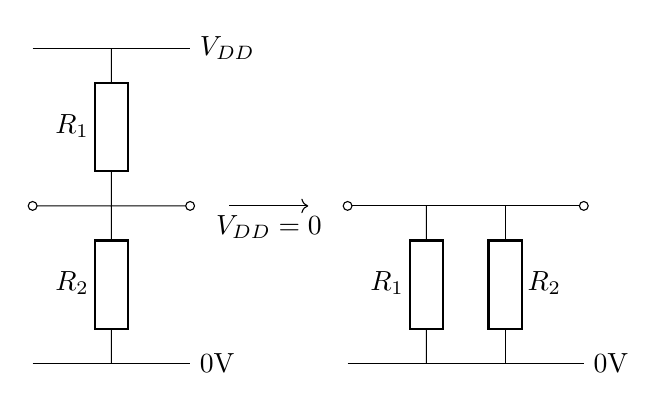
\begin{tikzpicture}
            %\draw[lightgray] (0, 0) grid (7, 4);
            \draw (0, 0) -- (2, 0) node[right] at (2, 0) {\SI{0}{V}};
            \draw (0, 4) -- (2, 4) node[right] at (2, 4) {\(V_{DD}\)};
            \draw (1, 0) to[R=\(R_2\)] (1, 2) to[short, -o] (0, 2);
            \draw (2, 2) to[short, o-] (1, 2) to[R=\(R_1\)] (1, 4);
            \draw [->] (2.5, 2) -- (3.5, 2) node[below] at (3, 2) {\(V_{DD} = 0\)};
            \draw (4, 2) to [short, o-o] (7, 2);
            \draw (5, 0) to[R=\(R_1\)] (5, 2);
            \draw (6, 2) to[R=\(R_2\)] (6, 0);
            \draw (4, 0) -- (7, 0) node[right] at (7, 0) {\SI{0}{V}};
        \end{tikzpicture}
        \caption{How series resistors can become parallel in a small signal model}
    \end{figure}
    
    If the values of \(R_C\) and the desired gain are specified then we can work out \(R_E\) using \(\text{gain} = -R_C/R_E\).
    We use
    \begin{equation}\label{eqn:V_BQ=V_DDR_2/(R_1+R_2)}
        V_{BQ} = V_{DD}\frac{R_2}{R_1 + R_2}
    \end{equation}
    to solve for \(R_2\) by substituting \(R_1 + R_2 = k(R_C + R_E)\) with some value of \(k\) that we decide is acceptable.
    We then choose the closest standard value for \(R_2\). Next we solve equation \ref{eqn:V_BQ=V_DDR_2/(R_1+R_2)} for \(R_1\) with our new value of \(R_2\).
    We the choose the next lower standard value for \(R_1\) (lower as current assumptions lead to an overestimate).
    
    \example
    Consider the circuit in figure \ref{fig:potential divider second voltage source}.
    We have the constraints that \(\text{gain} = -10\), \(R_C = \SI{10}{k\ohm}\) and \(V_{DD} = \SI{5}{V}\).
    What values should the other resistors take?
    \[\text{gain} = -\frac{R_C}{R_E}\implies R_E = -\frac{R_C}{\text{gain}} = -\frac{\SI{10}{k\ohm}}{-10} = \SI{1}{k\ohm}\]
    \[I_{C\text{min}} = \SI{0}{A}\]
    \[I_{C\text{max}} = \frac{V_{DD} - V_{CE\text{min}}}{R_C + R_E} = \frac{\SI{5}{V} - \SI{0.2}{V}}{\SI{10}{k\ohm} + \SI{1}{k\ohm}} = \SI{0.436}{mA}\]
    \[I_{CQ} = \frac{I_{C\text{min} + I_{C\text{max}}}}{2} = \frac{\SI{0}{A} + \SI{0.436}{mA}}{2} = \SI{0.218}{mA}\]
    \[V_{EQ} = I_{EQ}R_E\approx I_{CQ}R_E = \SI{0.218}{V}\]
    \[V_{BQ} = V_{CQ} + V_{EQ} = \SI{0.6}{V} + \SI{0.218}{V} = \SI{0.818}{V}\]
    \[V_{DD}\frac{R_2}{R_1 + R_2} = \SI{0.818}{V}\]
    \[V_{DD}\frac{R_2}{k(R_C + R_E)} = \SI{0.818}{V}\]
    We choose a value of \(k = 10\)
    \[\SI{5}{V}\frac{R_2}{10(\SI{10}{k\ohm} + \SI{1}{k\ohm})} = \SI{0.818}{V}\]
    \[R_2 = \SI{18}{k\ohm}\]
    This is a standard value already.
    Solving equation \ref{eqn:V_BQ=V_DDR_2/(R_1+R_2)} for \(R_1\) this time we get
    \[R_1 = \SI{92}{k\ohm}\]
    The next lower standard value is \SI{82}{k\ohm} so we use that.
    
    \section{Choosing Component Values}
    \begin{figure}[ht]
        \centering
        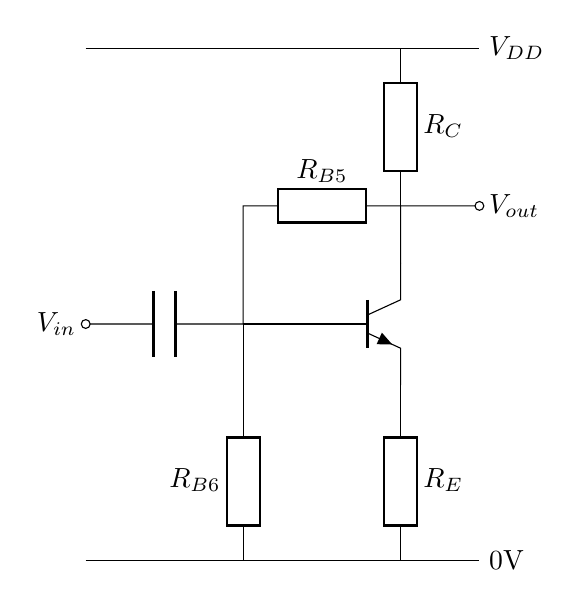
\begin{tikzpicture}
            %\draw[lightgray] (0, 0) grid (6, 7);
            \draw (0, 0) -- (5, 0) node[right] at (5, 0) {\SI{0}{V}};
            \draw (0, 3) to[C, o-] (2, 3) node[left] at (0, 3) {\(V_\text{in}\)};
            \draw (2, 0) to[R=\(R_{B6}\)] (2, 2) -- (2, 3);
            \node[npn](transistor) at (4, 3) {};
            \draw (2, 3) -- (transistor.base);
            \draw (transistor.emitter) -- (4, 2) to[R=\(R_E\)] (4, 0);
            \draw (2, 3) -- (2, 4.5) to[R=\(R_{B5}\)] (4, 4.5) -- (transistor.collector);
            \draw (4, 6.5) to[R=\(R_C\)] (4, 4.5);
            \draw (4, 4.5) to[short, -o] (5, 4.5) node[right] at (5, 4.5) {\(V_\text{out}\)};
            \draw (0, 6.5) -- (5, 6.5) node[right] at (5, 6.5) {\(V_{DD}\)};
        \end{tikzpicture}
        \caption{Circuit with unknown values}
        \label{fig:circuit with unknown values}
    \end{figure}
    The circuit in figure \ref{fig:circuit with unknown values} is part of a larger circuit which sets the following constraints: \(R_C = \SI{1}{k\ohm}\), \(\text{gain} = -10\) and \(V_{DD} = \SI{9}{V}\).
    We want to find suitable values for the other components.
    To do this we must consider the limitations of the circuit:
    \begin{itemize}
        \item To operate in a roughly linear manner we need \(R_E\gg r_\pi/\beta\), this means that we get \(|\text{gain}|\ll 100\), this is ok as we are only asking for \(\text{gain} = -10\).
        \item To have \(\text{gain}\approx -R_C/R_E\) we need \(R_{BE}\gg R_C\).
        \item To be independent of \(\beta\) we need \(R_{BE}\ll \beta(R_C + R_E)\).
    \end{itemize}
    The last two items are in direct contradiction so we must find a compromise.
    We start by calculating the value of \(R_E\):
    \[\text{gain} \approx-\frac{R_C}{R_E}\implies R_E\approx -\frac{R_C}{\text{gain}} = -\frac{\SI{1}{k\ohm}}{-10} = \SI{100}{\ohm}\]
    Next we calculate the quiescent current \(I_{CQ}\) through the collector.
    This is the average of the maximum and minimum currents \(I_{C\text{max}}\) and \(I_{C\text{min}}\).
    \[I_{C\text{min}} = \SI{0}{A}\]
    \[I_{C\text{max}} = \frac{V_{DD} - \SI{0.2}{V}}{R_C + R_E} = \frac{\SI{8.8}{V}}{\SI{1.1}{k\ohm}} = \SI{8}{mA}\]
    \[I_{CQ} = \frac{\SI{0}{A} + \SI{8}{mA}}{2} = \SI{4}{mA}\]
    Next we calculate the value of \(V_{EQ}\) using the fact that \(I_E = I_C + I_B\approx I_C\) as \(I_B\) is small
    \[V_{EQ} = I_{EQ}R_E\approx I_{CQ}R_E = \SI{4}{mA}\cdot\SI{100}{\ohm} = \SI{0.4}{V}\]
    Next we calculate the voltage drops \(V_{CQ}\) and \(V_{BQ}\):
    \[V_{CQ} = V_{DD} - I_{CQ}R_C\ = \SI{9}{V} - \SI{4}{mA}\cdot\SI{1}{k\ohm} = \SI{5}{V}\]
    \[V_{BQ} = V_{EQ} + \SI{0.6}{V} = \SI{0.4}{V} + \SI{0.6}{V} = \SI{1}{V}\]
    \(R_{B5}\) and \(R_{B6}\) form a potential divider, we can use this and the fact that the voltage at the base is \SI{1}{V}.
    \[V_{BQ} = V_{CQ}\frac{R_{B6}}{R_{B5} + R_{B6}}\]
    \[\SI{1}{V} = \SI{5}{V}\frac{R_{B6}}{R_B5} + R_{B6}\]
    \[R_{B5} + R_{B6}= 5R_B6\]
    \[R_{B5} = 4R_{B6}\]
    We choose a value of \(R_{B5}\) and check that our constraints hold.
    We choose \(R_{B5} = 10R_C = \SI{10}{k\ohm}\).
    First \(R_{BE}\gg R_C\) 
    \[\SI{10}{k\ohm}\gg \SI{1}{k\ohm}\]
    Second \(R_{BE} \ll \beta(R_C + R_E)\), we assume a value of \(\beta \approx 300\), this is the lower end of possible values for \(\beta\)
    \[\SI{10}{k\ohm} \ll 300\cdot\SI{1.1}{k\ohm} = \SI{330}{k\ohm}\]
    Satisfied that \(R_{B5} = \SI{10}{k\ohm}\) is reasonable we now calculate \(R_{B6}\)
    \[R_{B6} = \frac{R_{B5}}{4} = \frac{\SI{10}{k\ohm}}{4} = \SI{2.5}{k\ohm}\]
    This is not a standard value.
    We need to decide whether to round up or down to choose a standard value.
    The assumptions that we have made lead to lower voltage drop over \(R_{B6}\) than predicted so we choose to round up to fix this. 
    The next standard value is \(R_{B6} = \SI{2.7}{k\ohm}\).
    
    \subsection{Input and Output Impedances}
    Input and output impedances are important for small signals.
    Coupling capacitors form filters with the input and output impedances.
    The input impedance provides a load to the driving circuit, we want this to be high so that a high current is drawn.
    The output impedance provides a load to the transistor, we want this to be low so that there is more current for the circuit that we are driving.
    
    To find the output impedance \(R_\text{out}\) set \(V_\text{in} = 0\) and inject current \(i_o\) into the output then calculate the resistance as
    \[R_\text{out} = \frac{V_\text{out}}{i_o}\]
    Consider the small signal model in figure \ref{fig:small signal output impedance} by setting the input voltage to 0 we get the circuit in figure \ref{fig:0 input output impedence}
    
    \begin{figure}[ht]
        \centering
        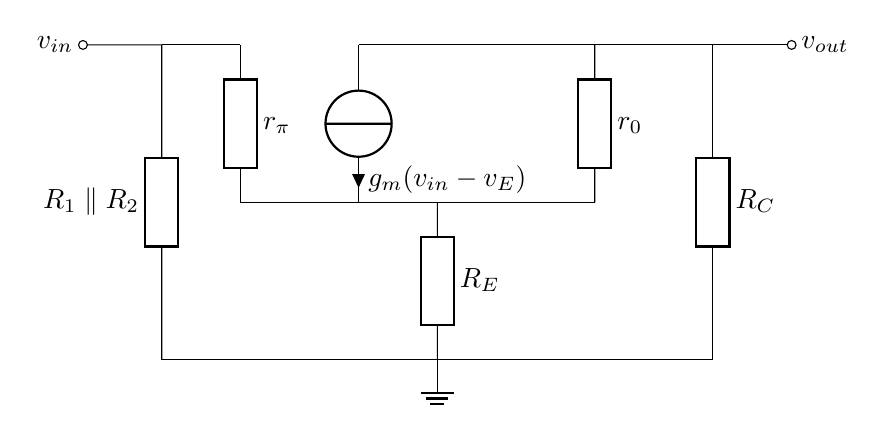
\begin{tikzpicture}
            %\draw[lightgray] (0, 0) grid (8, 4);
            \draw (1, 0) to[R=\(R_1\parallel R_2\)] (1, 4) to[short, -o] (0, 4) node[left] at (0, 4) {\(v_\text{in}\)};
            \draw (2, 4) to[R=\(r_\pi\)] (2, 2);
            \draw (3.5, 4) to[I=\(g_m(v_\text{in} - v_E)\)] (3.5, 2);
            \draw (6.5, 4) to[R=\(r_0\)] (6.5, 2);
            \draw (8, 4) to[R=\(R_C\)] (8, 0);
            \draw (4.5, 2) to[R=\(R_E\)] (4.5, 0);
            \draw (8, 4) to[short, -o] (9, 4) node[right] at (9, 4) {\(v_\text{out}\)};
            \node[ground] at (4.5, 0) {};
            \draw (1, 0) -- (8, 0);
            \draw (2, 2) -- (6.5, 2);
            \draw (1, 4) -- (2, 4);
            \draw (3.5, 4) -- (8, 4);
        \end{tikzpicture}
        \caption{Small signal model to calculate output impedance}
        \label{fig:small signal output impedance}
    \end{figure}

        \begin{figure}[ht]
        \centering
        \begin{tikzpicture}
        %\draw[lightgray] (0, 0) grid (8, 4);
        \draw (1, 0) to[R=\(R_1\parallel R_2\)] (1, 4) -- (-0.6, 4) -- (-0.6, 0) -- (1, 0);
        \draw (2, 4) to[R=\(r_\pi\)] (2, 2);
        \draw (3.5, 4) to[I=\(g_m(v_\text{in} - v_E)\)] (3.5, 2);
        \draw (6.5, 4) to[R=\(r_0\)] (6.5, 2);
        \draw (8, 4) to[R=\(R_C\)] (8, 0);
        \draw (4.5, 2) to[R=\(R_E\)] (4.5, 0);
        \draw (9, 4) to[short, o-, i=\(i_o\)] (8, 4) node[right] at (9, 4) {\(v_\text{out}\)};
        \node[ground] at (4.5, 0) {};
        \draw (1, 0) -- (8, 0);
        \draw (2, 2) -- (6.5, 2);
        \draw (1, 4) -- (2, 4);
        \draw (3.5, 4) -- (8, 4);
        \end{tikzpicture}
        \caption{Small signal model with input voltage set to 0}
        \label{fig:0 input output impedence}
    \end{figure}
    We can then analyse the circuit to find out the output impedance
    \[(0-v_E)g_\pi + (0-v_E)g_m + (v_\text{out}-v_E)g_0 + (0-v_E)G_E = 0\]
    \[\implies g_0v_\text{out} = v_E(g_pi + g_m + g_0 + G_E)\]
    \[-g_m(0-v_E) + (v_E-v_\text{out}) + G_0(0-v_\text{out}) + i_o\]
    \[\implies v_\text{out}(g_0 + G_C) - i_o = v_E(g_0 + g_,)\]
    Eliminate \(v_E\) and substitute \(R_\text{out} = v_\text{out}/i_o\) to get
    \[R_\text{out} = \frac{g_\pi + g_m + g_0 + G_C}{g_0(g_\pi + G_E) + G_C(g_\pi + g_m + g_0 + G_E)}\]
    Looking at typical values we see that the term containing \(g_m\) is dominant so we can ignore the term \(g_0(g_\pi + G_E)\) which simplifies the equation to
    \[R_\text{out}\approx \frac{1}{G_C} = R_C\]
    
    To find the input impedance we first consider the input impedance \(R_\text{inT}\) without \(R_1\parallel R_2\).
    We can do this using \(R_\text{inT} = v_\text{in}/i_B\) where \(i_B\) is the current at the base.
    We use \(i_B = (v_\text{in} - v_E)/r_\pi\) and we solve the same equations as before but eliminate \(v_\text{out}\).
    We get
    \[R_\text{inT} = \frac{g_0(g_\pi + G_E + G_C) + G_C(g_\pi + g_m + G_E)}{g_\pi(g_0G_E + g_0G_C + G_CG_E)}\]
    We can assume \(g_0\approx 0\) as \(r_0\) is large
    \[R_\text{inT}\approx \frac{g_\pi + g_m + G_E}{g_\pi G_E}\]
    We can substitute \(g_m \beta g_\pi\)
    \[R_\text{inT} = \frac{g_\pi + \beta g_\pi + G_E}{g_\pi G_E} = \left(1 + \beta + \frac{G_E}{g_\pi}\right)R_E = (1 + \beta)R_E + r_\pi\]
    The overall input impedance is
    \[R_\text{in} = R_\text{inT}\parallel R_1\parallel R_2\]
    For good DC bias stability we need \(R_1\parallel R_2\) to be low so this term dominates \(R_\text{in}\) however we wanted a large input impedance.
    
    One solution is to have an inductor between \(R_1\) and the base as well as the existing connection and then also a capacitor between the input and the rest of the circuit.
    This is common for radio frequencies but at audio frequencies the inductor needed is physically too large for most applications.
    
    Another solution is to short \(R_E\) to AC gain, this means connecting a capacitor from between the emitter and \(R_E\) and ground, call this capacitor \(C_E\) and it has impedance \(Z_E\).
    We define \(Z_{Em} = R_E\parallel Z_E\) if \(C_E\) is large then \(Z_E\) is small at high frequencies so \(Z_{Em}\) is small even at medium frequencies
    This gives us
    \[\lim_{Z_{Em}\to 0}-\frac{R_C}{Z_{Em}} = -\infty\]
    Clearly this isn't physically true, what is actually happening is that \(G_E\) is going to \(\infty\) which means that the AC gain in equation \ref{eqn:gain=-gm?(g0+GC)} goes to
    \[\text{gain} = \frac{g_m}{g_0+ G_C}\]
    This is very dependent on \(\beta\) and is non-linear.
    The magnitude of gain is now much larger than \(R_C/R_E\).
    To find the values of the gain, \(R_\text{out}\) and \(R_\text{in}\) we set \(R_E = 0\) and do the analysis.
    This gives amongst other results \(R_\text{inT} = (\beta + 1)R_E + r_\pi = r_\pi\). This means that we can't just ignore \(r_\pi\) as we often would.
    This circuit has good DC stability bias but the full gain of the circuit with \(R_E = 0\).
    The non-linear nature of this circuit makes it only useful for very small signals such as the first signals picked up by a radio antenna before they are amplified.
    
    \section{Common Amplifiers}
    Figure \ref{fig:negative feedback} shows a common emitter amplifier.
    It gets this name from the fact that the emitter is `shared' between the input and output as input is developed over the base and emitter and output is developed over the collector and emitter.
    It has a small signal voltage as an input and its output is an amplified voltage.
    The gain is controlled by \(\beta\) and \(g_m = I_C/V_T\).
    It has high gain but is very non-linear.
    
    \begin{figure}[ht]
        \centering
        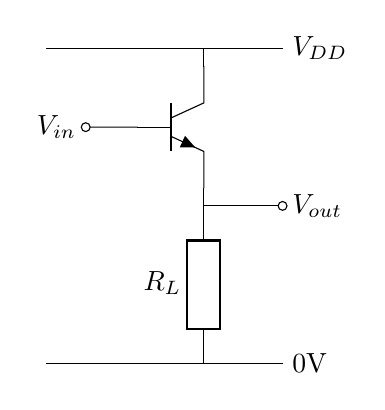
\begin{tikzpicture}
            %\draw[lightgray] (0, 0) grid (3, 4);
            \draw (0, 0) -- (3, 0) node[right] at (3, 0) {\SI{0}{V}};
            \draw (2, 0) to[R=\(R_L\)] (2, 2);
            \node[npn](transistor) at (2, 3) {};
            \draw (transistor.emitter) -- (2, 2);
            \draw (transistor.base) to[short, -o] (0.5, 3) node[left] at (0.5, 3) {\(V_\text{in}\)};
            \draw (transistor.collector) -- (2, 4);
            \draw (2, 2) to[short, -o] (3, 2) node[right] at (3, 2) {\(V_\text{out}\)};
            \draw (0, 4) -- (3, 4) node[right] at (3, 4) {\(V_{DD}\)};
        \end{tikzpicture}
        \caption{Common collector amplifier}
        \label{fig:common collector amplifier}
    \end{figure}

    Figure \ref{fig:common collector amplifier} shows a common collector amplifier (also known as an emitter follower).
    The collector is shared between the input and output, there is no collector resistor.
    The output is attached to the emitter which is at diode voltage (\(\sim\SI{0.6}{V}\)) below the base.
    This value is basically constant so there is no voltage amplification, however there is current amplification as the current \(I_C\) at the emitter is \(I_B + IC\).
    This circuit is used to drive circuits requiring high currents.
    It may need a heat sink.
    
    \begin{figure}[ht]
        \centering
        \begin{tikzpicture}
            %\draw[lightgray] (0, 0) grid (7, 5);
            \draw (0, 3) to[C, o-] (2, 3) node[left] at (0, 3) {\(V_\text{in}\)};
            \draw (2, 3) to[R=\(R_{B1}\)] (2, 0);
            \draw (0, 0) -- (7, 0) node[right] at (7, 0) {\(V_{SS}\)};
            \node[npn, rotate=-90, xscale=-1](transistor) at (4, 3) {};
            \draw (transistor.emitter) -- (2, 3);
            \draw (transistor.base) -- (4, 1) node[ground] at (4, 1) {};
            \draw (transistor.collector) to[C, -o] (7, 3) node[right] at (7, 3) {\(V_\text{out}\)};
            \draw (5, 3) to[R=\(R_C\)] (5, 5);
            \draw (0, 5) -- (7, 5) node[right] at (7, 5) {\(V_{DD}\)};
        \end{tikzpicture}
        \caption{Common base amplifier}
        \label{fig:common base amplifier}
    \end{figure}

    Figure \ref{fig:common base amplifier} shows a common base amplifier.
    This circuit avoids the Miller effect (accidental creation of a capacitance between input and output).
    The current gain is less than 1, it is about 0.98.
    There is no or little voltage gain.
    It has a small input impedance and large output impedance.
    This lets it act as a current buffer.
    The emitter voltage must (for an NPN transistor) be below the base voltage for the current to flow so for this circuit \(V_E\) is negative.
    
    \subsection{Amplifier Model}
    The circuit shown in figure \ref{fig:potential divider second voltage source} can be modelled by a perfect amplifier with gain \(G\) and two resistors to model input and output impedance such as in figure \ref{fig:amplifier model}
    
    \begin{figure}[ht]
        \centering
        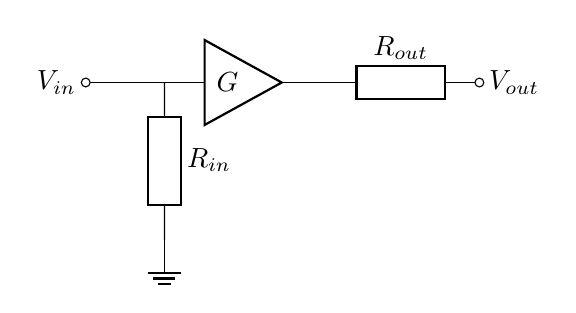
\begin{tikzpicture}
            \draw (0, 2) to[short, o-] (1, 2) node[left] at (0, 2) {\(V_\text{in}\)};
            \draw (1, 2) to[R=\(R_\text{in}\)] (1, 0) node[ground] at (1, 0) {};
            \draw (1, 2) to[amp] (3, 2);
            \node at (1.8, 2) {\(G\)};
            \draw (3, 2) to[R=\(R_\text{out}\), -o] (5, 2) node[right] at (5, 2) {\(V_\text{out}\)};
        \end{tikzpicture}
        \caption{Amplifier model}
        \label{fig:amplifier model}
    \end{figure}
    
    \(G \approx -R_C/R_E\), \(R_\text{in}\approx R_1\parallel R_2\parallel (\beta + 1)R_E\) and \(R_\text{out}\approx R_C\).
    Two such circuits can be chained together such as in figure \ref{fig:double amplifier model} with source resistance \(R_S\) and load resistance \(R_L\). They will have gain
    \[\frac{V_\text{out}}{V_\text{in}} = G_1G_2\frac{R_\text{in1}}{R_S + R_in1}\frac{R_\text{in2}}{R_\text{out1} + R_\text{in2}}\frac{R_L}{R_{out2}+R_L} \ll G_1G_2\]
    \begin{figure}[ht]
        \centering
        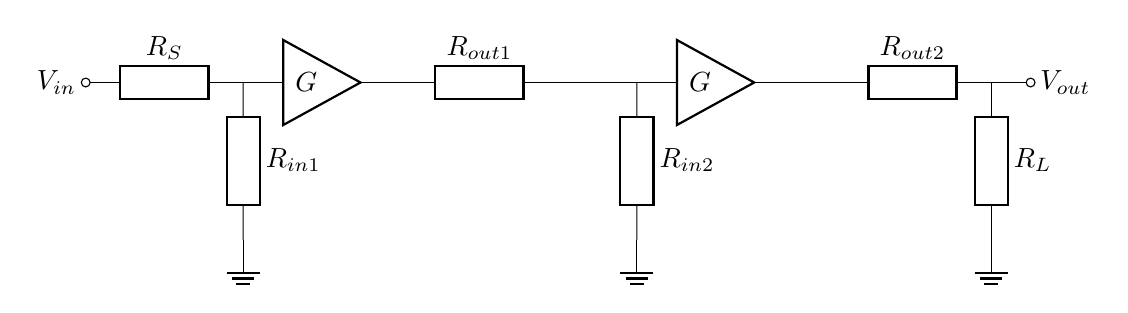
\begin{tikzpicture}
            \draw (-1, 2) to[R=\(R_S\), o-] (1, 2) node[left] at (-1, 2) {\(V_\text{in}\)};
            \draw (1, 2) to[R=\(R_\text{in1}\)] (1, 0) node[ground] at (1, 0) {};
            \draw (1, 2) to[amp] (3, 2);
            \node at (1.8, 2) {\(G\)};
            \draw (3, 2) to[R=\(R_\text{out1}\)] (5, 2);
            \begin{scope}[xshift=5cm]
                \draw (0, 2) to[short] (1, 2);
                \draw (1, 2) to[R=\(R_\text{in2}\)] (1, 0) node[ground] at (1, 0) {};
                \draw (1, 2) to[amp] (3, 2);
                \node at (1.8, 2) {\(G\)};
                \draw (3, 2) to[R=\(R_\text{out2}\), -o] (6, 2) node[right] at (6, 2) {\(V_\text{out}\)};
                \draw (5.5, 2) to[R=\(R_L\)] (5.5, 0) node[ground] at (5.5, 0) {};
            \end{scope}
        \end{tikzpicture}
        \caption{Amplifiers in series}
        \label{fig:double amplifier model}
    \end{figure}

    \section{Impedance}
    Ideal resistors have a flat frequency response, that is they have the same effect at all frequencies.
    Capacitors and inductors have different effects on different frequencies.
    Frequency dependent responses can be modelled as impedances which are frequency dependent resistances.
    Angular frequency \(\omega = 2\pi f\) is commonly used.
    The impedance \(Z_C\) of a capacitor is
    \[Z_C = \frac{1}{j\omega C}\]
    where \(j^2 = -1\).
    The impedance \(Z_L\) of an inductor is
    \[Z_L = j\omega L\]
    These can be used in calculations the same way that resistances are.
    \begin{figure}[ht]
        \centering
        \begin{tikzpicture}
            \draw (0, 2) to[R=\(R\), o-] (2, 2) node[left] at (0, 2) {\(V_\text{in}\)};
            \draw (2, 2) to[C=\(C\)] (2, 0) node[ground] at (2, 0) {};
            \draw (2, 2) to[short, -o] (2.5, 2) node[right] at (2.5, 2) {\(V_\text{out}\)};
        \end{tikzpicture}
        \caption{A resistor and capacitor make a potential divider}
        \label{fig:resistor-capacitor potential divider}
    \end{figure}
    Consider the circuit in figure \ref{fig:resistor-capacitor potential divider}. 
    The resistor and capacitor form a parallel divider.
    The output voltage can hence be calculated as
    \[V_\text{out} = V_\text{in}\frac{Z_C}{R + Z_C} = V_\text{in}\frac{\frac{1}{j\omega C}}{R + \frac{1}{j\omega C}} = V_\text{in}\frac{1}{j\omega CR + 1}\]
    \[\omega \ll \frac{1}{CR}\implies \text{gain}\approx 1\]
    \[\omega \gg \frac{1}{CR}\implies \text{gain}\approx 0\]
    This actually defines what we think of as AC and DC for our circuit, this is a low pass filter as only the low frequencies can get through.
    Anything that makes it through this we think of as DC, likewise anything that makes it through a high pass filter (just a capacitor) we think of as AC.
    
    If we include a decoupling capacitor \(C_\text{in}\) and a load capacitor \(C_L\) to our circuit in figure \ref{fig:amplifier model} we get the circuit if figure \ref{fig:amplifier model with capacitors}
    \begin{figure}[ht]
        \centering
        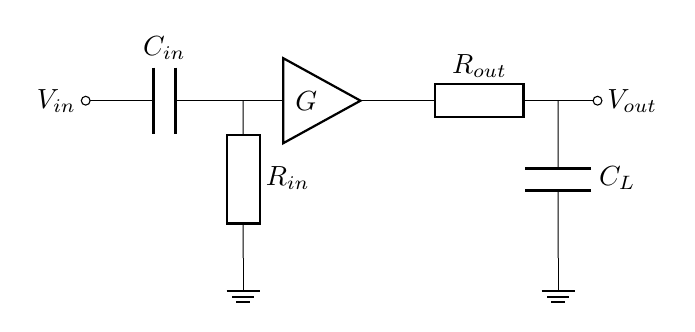
\begin{tikzpicture}
            \draw (-1, 2) to[C=\(C_\text{in}\), o-] (1, 2) node[left] at (-1, 2) {\(V_\text{in}\)};
            \draw (1, 2) to[R=\(R_\text{in}\)] (1, 0) node[ground] at (1, 0) {};
            \draw (1, 2) to[amp] (3, 2);
            \node at (1.8, 2) {\(G\)};
            \draw (3, 2) to[R=\(R_\text{out}\)] (5, 2) to[short, -o] (5.5, 2) node[right] at (5.5, 2) {\(V_\text{out}\)};
            \draw (5, 2) to[C=\(C_L\)] (5, 0) node[ground] (5, 0) {};
        \end{tikzpicture}
        \caption{Amplifier with capacitors}
        \label{fig:amplifier model with capacitors}
    \end{figure}
    The gain as a function of frequency is
    \[\text{gain}(\omega) = \frac{j\omega R_\text{in}C_\text{in}}{1 + j\omega R_\text{in}C_\text{in}}G\frac{1}{1 + j\omega R_\text{out}C_L}\]
    The first term goes to 0 for low values of \(\omega\) and 1 for high values of \(\omega\).
    This limits the frequencies over which we actually get the calculated gain.
    We tend to get the expected gain in the region of \SIrange{10}{e5}{Hz}. Either side of this the gain decreases as you get further from this range.
    
    Phase is also affected by the capacitors.
    Below \SI{10}{Hz} the phase change is \SI{-90}{\SIUnitSymbolDegree}.
    From \SIrange{10}{e5}{Hz} the phase change is \SI{-180}{\SIUnitSymbolDegree}.
    Above \SI{e5}{Hz} the phase change is \SI{-270}{\SIUnitSymbolDegree}.
    
    All of these are just rules of thumb as the values actually change much more smoothly with frequency.
    
    \section{Bode Plots}
    All AC analogue circuits have a frequency response.
    The circuit transfer function is defined as \(G(\omega) = V_\text{out}/V_\text{in}\).
    Output signals will have a different amplitude and phase but the same frequency \(f\).
    Bode plots plot the magnitude or phase of the transfer function against (log) frequency (usually angular frequency \(\omega = 2\pi f\)).
    The gain is usually measured in decibels \si{dB}.
    It is defined as
    \[\text{gain} = 10\log_{10}\left(\frac{P_\text{out}}{P_\text{in}}\right)\,\si{dB}\]
    using \(P = V^2/R\) we get
    \[\text{gain} = 10\log_{10}\left(\frac{V_\text{out}^2/R_\text{out}}{V_\text{in}^2/R_\text{in}}\right)\,\si{dB} = 20\log_{10}\left(\frac{V_\text{out}}{V_\text{in}}\right)\,\si{dB}\]
    assuming that \(R_\text{out} = R_\text{in}\).
    Gains in decibels are added together whereas linear gains are multiplied.
    \begin{table}[ht]
        \centering
        \begin{tabular}{|c|c|c||c|c|}\hline
            Linear Gain & Approximate Gain & Accurate Gain & Linear Gain &  Accurate Gain\\
            (-) & (\si{dB}) & (\si{dB}) & (-) & (\si{dB})\\ \hline
            2 & 6 & 6.0206 & 10 & 20\\ \hline
            3 & 10 & 9.5424 & 100 & 40\\ \hline
            5 & 14 & 13.9794 & 100 & 60\\ \hline
        \end{tabular}
        \caption{Some common values of gain}
        \label{tab:common gains}
    \end{table}
    Table \ref{tab:common gains} shows some values of common gains.
    These are useful for doing conversions for example:
    \[150 = 3\cdot 5 \cdot 10\to \SI{10}{dB} + \SI{14}{dB} + \SI{20}{dB} = \SI{44}{dB}\]
    \[\SI{36}{dB} = \SI{20}{dB} + \SI{10}{dB} + \SI{6}{dB} = 10 \cdot 3 \cdot 2 = 60\]
    Note that \(\SI{0}{dB} = 1\) and \(\log_{10}(1/x) = -\log_{10}(x)\) so, for example a gain of \(0.1 = 1/10 = -\SI{20}{dB}\).
    
    \subsection{Bode Plot of a Low Pass Filter}
    \begin{figure}[ht]
        \centering
        \begin{tikzpicture}
            \draw (0, 0) to[V=\(V_\text{in}(t)\)] (0, 2);
            \draw (0, 2) to[R=\(R\)] (2, 2);
            \draw (2, 0) to[C=\(C\), v=\(V_\text{out}(t)\)] (2, 2);
            \draw (2, 0) -- (0, 0);
        \end{tikzpicture}
        \caption{Low pass filter}
        \label{fig:low pass filter}
    \end{figure}
    
    Figure \ref{fig:low pass filter} shows a low pass filter.
    The resistor and capacitor form a parallel divider so we can calculate \(V_\text{out}\) as a function of \(V_\text{in}\).
    \[V_\text{out} = V_\text{in}\frac{\frac{1}{j\omega C}}{R + \frac{1}{j\omega C}}\]
    \[G(\omega) = \frac{V_\text{out}}{V_\text{in}} = \frac{1}{1 + j\omega RC} = \frac{1}{1 + j\omega \tau}\]
    where \(\tau = RC\) is the circuits time constant in seconds.
    
    The amplitude (or magnitude) response is given by the modulus of the transfer function
    \[|G(\omega)| = \left |\frac{V_\text{out}}{V_\text{in}}\right | = \left |\frac{1}{1 + j\omega \tau}\right | = \frac{1}{\sqrt{1 + (\omega\tau)^2}}\]
    The amplitude Bode plot is \(\log_{10}(\omega)\) against \(|G(\omega)|\) and is shown in figure \ref{fig:bode amplitude plot LPF}.
    \begin{figure}[ht]
        \centering
        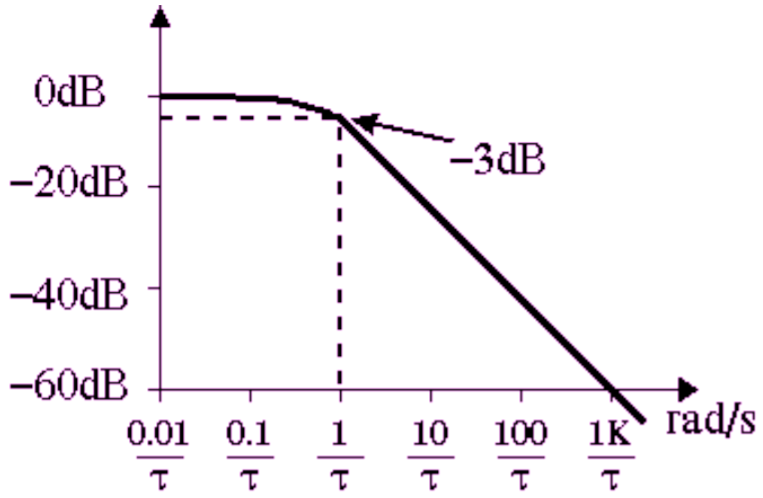
\includegraphics[scale=0.3]{amplitude_bode_plot_low_pass_filter.png}
        \caption{The amplitude Bode plot for a low pass filter}
        \label{fig:bode amplitude plot LPF}
    \end{figure}
    This drops rapidly at~\(\omega = 1/\tau\)
    \[\left |G\left(\frac{1}{\tau}\right)\right | = \frac{\sqrt{2}}{2}\xrightarrow[\si{dB}]{} 20\log_{10}\left(\frac{\sqrt 2}{2}\right) = -\SI{3}{dB}\]
    A signal at frequency \(\omega = 1/\tau\) will be attenuated by \SI{3}{dB}.
    This is known as the \SI{3}{dB} cut off point and marks the edge of the passband (where we say things pass the filter vs where they are blocked).
    
    The passband of a filter is defined as the frequency band between two half power units.
    That is the range of frequencies where the power out is at least half the power in.
    Since \(P = V^2/R\) at half power
    \[\frac{P}{2} = \frac{V^2}{2R} = \frac{(V^2/\sqrt{2})}{R}\]
    so at half power the voltage is attenuated by \(\sqrt{2}\).
    For a low pass filter the upper cut off is at \(-\SI{3}{dB}\) and the lower cut off is at \(\omega = \SI{0}{s^{-1}}\).
    The stopband is anywhere not in the pass band so for a low pass filter it is at \(\omega \ge 1/\tau\)
    
    The phase response of a gain function \(G(\omega) = n(\omega)/d(\omega)\) where \(n, d:\bb C\to\bb C\) is given by:
    \[\arg(G(\omega)) = \arctan\left(\frac{\Im(n(\omega))}{\Re(n(\omega))}\right) - \arctan\left(\frac{\Im(d(\omega))}{\Re(d(\omega)}\right)\]
    so for a low pass filter
    \[\arg(G(\omega)) = \arg\left(\frac{1}{1 + j\omega \tau}\right) = \arctan\left(\frac{0}{1}\right) - \arctan\left(\frac{\omega\tau}{1}\right) = -\arctan(\omega\tau)\]
    Evaluating at the same point, \(\omega = 1/\tau\), as before we get
    \[\arg\left(G\left(\frac{1}{\tau}\right)\right) = -\arctan(1) = -\frac{\pi}{4}\]
    or evaluating at \(\omega = 0\):
    \[\arg(G(0)) = -\arctan(0) = 0\]
    We can also consider the nature of this as \(\omega \to \infty\) and we see that
    \[\lim_{\omega\to\infty}\arg(G(\omega)) = \lim_{\omega\to\infty}-\arctan(\omega\tau) = -\frac{\pi}{2}\]
    Plotting this function on logarithmic axes gives the plot shown in figure \ref{fig:bode phase plot LPF}
    \begin{figure}[ht]
        \centering
        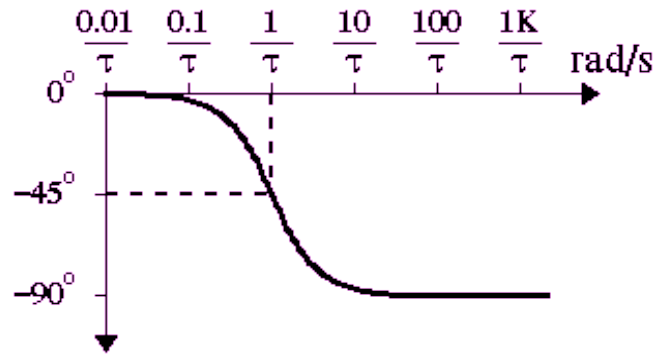
\includegraphics[scale=0.3]{phase_bode_plot_low_pass_filter.png}
        \caption{The phase Bode plot of a low pass filter}
        \label{fig:bode phase plot LPF}
    \end{figure}
    
    \subsection{Approximation to Straight Lines}
    So far we have considered plots of smooth, continuous functions.
    It is often favourable to approximate these with some line segments instead.
    Here we will do this for a low pass filter to show how it is done.
    
    At high frequencies we take \(\omega_1 \gg \frac{1}{\tau}\) we also let \(\omega_2 = 10\omega_1\).
    The curve between these two points on the amplitude bode plot can be considered a straight line.
    \[G_{\si{dB}}(\omega_1) = 20\log_{10}\left(\frac{1}{\omega_1\tau}\right) = -20\log_{10}(\omega_1) - 20\log_{10}(\tau)\]
    \begin{align*}
        G_{\si{dB}}(\omega_2) &= 20\log_{10}\left(\frac{1}{\omega_2\tau}\right)\\
        &= -20\log_{10}(\omega_2) - 20\log_{10}(\tau)\\
        &= -20\log_{10}(10\omega_1) - 20\log_{10}(\tau)\\
        &= -20 -20\log_{10}(\omega_1) - 20\log_{10}(\tau)\\
        &= -20 + G_{\si{dB}}(\omega_1)
    \end{align*}
    This means that our function has a slope of \(-\SI{20}{dB}\) per decade (10 fold increase).
    The first approximation we can make is that for input frequencies higher than \(1/\tau\) we can approximate the curve as a linear segment with a slope of \(-\SI{20}{dB}\) per decade.
    
    \[\lim_{\omega\to 0}|G(\omega)| = 1\]
    so for low frequencies less than \(1/\tau\) we can approximate the curve as a flat line with a linear gain of 1 which is a gain of \SI{0}{dB}.
    Making both of these approximations gives us the graph shown in figure \ref{fig:amplitude bode plot LPF approx}. The maximum error is at the passband cut off where we approximate as \SI{0}{dB} but it is actually \(-\SI{3}{dB}\)
    \begin{figure}[ht]
        \centering
        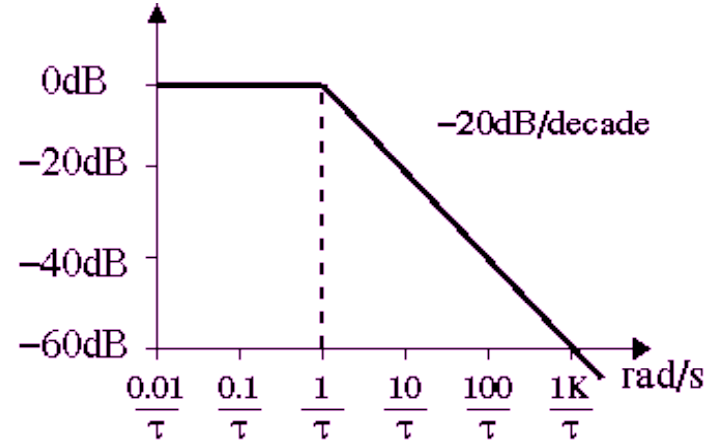
\includegraphics[scale=0.3]{approx_amplitude_bode_plot_low_pass_filter.png}
        \caption{Approximate amplitude Bode plot of a low pass filter}
        \label{fig:amplitude bode plot LPF approx}
    \end{figure}
    Likewise for the phase Bode plot we can make the following approximations:
    \begin{itemize}
        \item \SI{0}{\SIUnitSymbolDegree} for \(\omega < 0.1/\tau\)
        \item Straight line slope \SI{-45}{\SIUnitSymbolDegree} per decade for \(0.1/\tau < \omega < 10/\tau\)
        \item \SI{-90}{\SIUnitSymbolDegree} for \(\omega > 10/\tau\)
    \end{itemize}
    This gives the graph in figure \ref{fig:phase bode plot LPF approx}. The maximum error occurs at \(\omega = 0.1/\tau\) and \(\omega = 10/\tau\)
    \begin{figure}[ht]
        \centering
        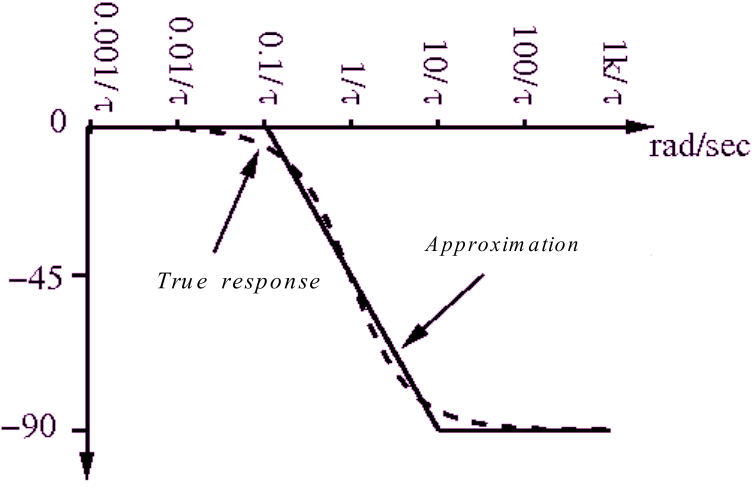
\includegraphics[scale=0.3]{approx_phase_bode_plot_low_pass_filter.png}
        \caption{Approximate phase Bode plot of a low pass filter}
        \label{fig:phase bode plot LPF approx}
    \end{figure}
        
    \section{Bode Plots of Simple Functions}
    It is often easier to split a function into several simple cases which can be combined. Some useful functions are given below
    \[G(\omega) = k\text{ where }k\in\bb R\]
    \[|G(\omega)| = |k|\]
    \[|G(\omega)|_{\si{dB}} = 20\log_{10}(k)\]
    Amplitude Bode plot - a horizontal line at \(20\log_{10}(k)\).
    \[\arg(G(\omega)) = \arctan\left(\frac{0}{k}\right) = 0\]
    Phase Bode plot - a horizontal line at 0.
    \[G(\omega) = j\omega\]
    \[|G(\omega)| = \omega\]
    \[|G(\omega)|_{\si{dB}} = 20\log_{10}(\omega)\]
    At \(\omega = 10\omega_0\):
    \[|G(\omega)|_{\si{dB}} = 20\log_{10\omega_0} = 20 + 20\log_{10}(\omega_0)\]
    The magnitude response has a \SI{20}{dB} per decade slope that goes through \((0, 0)\).
    \[\arg(G(\omega)) = \arctan\left(\frac{\omega}{0}\right) = \arctan(\infty) = \SI{90}{\SIUnitSymbolDegree}\]
    The phase response is a horizontal line at \SI{90}{\SIUnitSymbolDegree}
    \[G(\omega) = 1 + j\omega\tau\]
    This is the inverse of the low pass filter from the previous section.
    Since \(\log(1/x) = -\log(x)\) the amplitude response is the same as for the low pass filter but flipped in the frequency axis.
    \[\arg(G(\omega)) = \arctan\left(\frac{\omega\tau}{1}\right) = \arctan(\omega\tau)\]
    This is 0 for low \((<0.1/\tau)\) values of omega and \SI{90}{\SIUnitSymbolDegree} for high \((>10/\tau)\) values of omega.
    
    For more complex transfer functions we can split them into a product of the above functions and the transfer function of a low pass filter.
    This then becomes a product in the log domain.
    Say a transfer function \(G\) can be split into \(n\) transfer functions \(G_i\), like the above examples, we then have
    \[G(\omega) = \prod_{i=1}^{n}G_i(\omega) = \sum_{i=1}^{n}G_i(\omega)_{\si{dB}}\]
    The phases just add as multiplying complex numbers just adds the phases:
    \[re^{j\vartheta} \cdot se^{j\varphi} = rse^{i(\vartheta + \varphi)}\]
    
    \example
    \[G(\omega) = \frac{2j\omega(10^4 + j\omega)}{(10 + j\omega)(10^7 + j\omega)}\]
    \[G(\omega) = [2][j\omega][10^4+j\omega]\left[\frac{1}{10 + j\omega}\right]\left[\frac{1}{10^7 + j\omega}\right]\]
    Collecting all of the constants we get
    \[G(\omega) = \underbrace{[2\cdot 10^{-4}]}_{G_1(\omega)} \underbrace{[j\omega]}_{G_2(\omega)} \underbrace{[1 + 10^{-4}j\omega]}_{G_3(\omega)} \underbrace{\left[\frac{1}{1 + 10^{-1}j\omega}\right]}_{G_4(\omega)} \underbrace{\left[\frac{1}{1 + 10^{-7}j\omega}\right]}_{G_5(\omega)}\]
    Adding together all of the Bode plots for all \(G_i\) gives the Bode plot shown in figure \ref{fig:complex bode plot}
    \begin{figure}[ht]
        \centering
        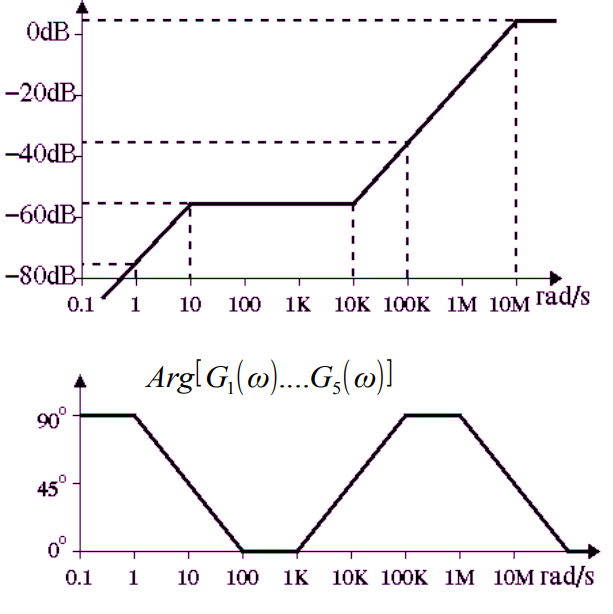
\includegraphics[scale=0.4]{complex_bode_plot.png}
        \caption{The resulting Bode plot}
    \end{figure}

    \section{Filter Bode Plots}
    \subsection{High Pass Filter}
    \begin{figure}[ht]
        \centering
        \begin{tikzpicture}
            \draw (0, 0) to[V=\(V_\text{in}(t)\)] (0, 2);
            \draw (0, 2) to[C=\(C\)] (2, 2);
            \draw (2, 0) to[R=\(R\), v=\(V_\text{out}(t)\)] (2, 2);
            \draw (2, 0) -- (0, 0);
        \end{tikzpicture}
        \caption{A high pass filter}
        \label{fig:high pass filter}
    \end{figure}
    A high pass filter is constructed as in figure \ref{fig:high pass filter}.
    Treating it as  a potential divider we see
    \[V_\text{out} = \frac{R}{R + \frac{1}{j\omega C}}V_\text{in}\]
    This gives us
    \begin{align*}
        G(\omega) &= \frac{j\omega \tau}{1 + j\omega \tau}\\
        &= [\tau][j\omega]\left[\frac{1}{1 + j\omega\tau}\right]
    \end{align*}
    This gives the Bode plots shown in figure \ref{fig:bode plots HPF}
    \begin{figure}[ht]
        \centering
        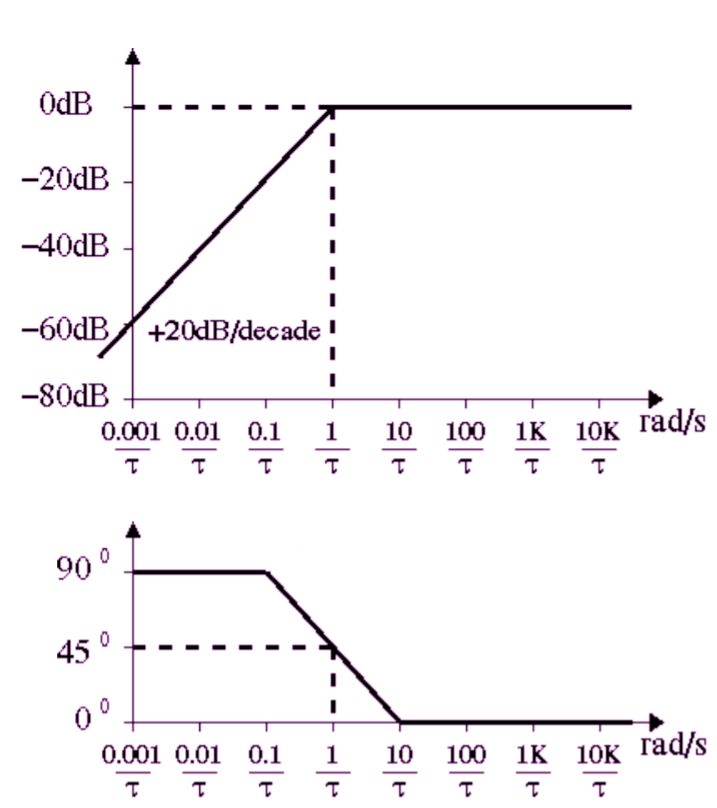
\includegraphics[scale=0.6]{HPF_bode_plot.png}
        \caption{Bode plots for a high pass filter}
        \label{fig:bode plots HPF} 
    \end{figure}
    
    \subsection{Phase Shifter}
    A useful transfer function is
    \[G(\omega) = \frac{1 - j\omega\tau}{1 + j\omega \tau} = \underbrace{[1 + j\omega\tau]}_{G_1(\omega)} \underbrace{\left[\frac{1}{1 + j\omega\tau}\right]}_{G_2(\omega)}\]
    \(G_1(\omega)\) is the transfer function of a low pass filter.
    \[|G_2(\omega)| = |1 - j\omega\tau| = \sqrt{1 + (\omega\tau)^2}\]
    This is the same as an inverted low pass amplitude response
    \[\arg(G_2(\omega)) = \arctan\left(\frac{-\omega\tau}{1}\right) = \arctan(\omega\tau)\]
    This is the same as the low pass response.
    Plotting the Bode plots gives figure \ref{fig:phase shifter bode plot}.
    You can see that the magnitude responses cancel to a gain of \SI{0}{dB} and the phase is bounded between \SIlist{0;90}{\SIUnitSymbolDegree}.
    \begin{figure}[ht]
        \centering
        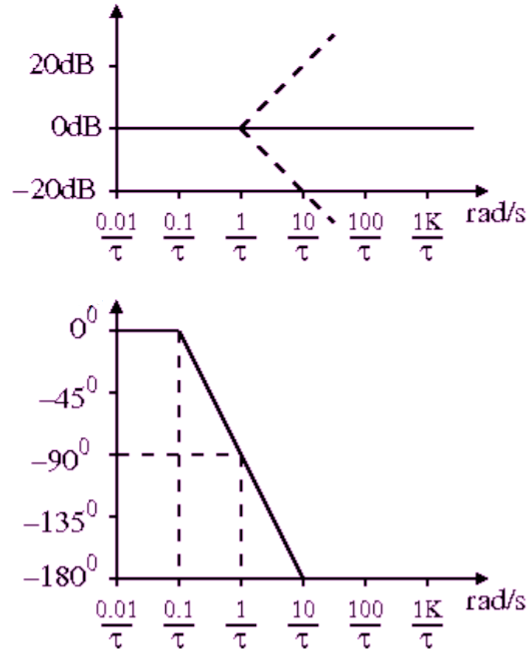
\includegraphics[scale=0.4]{phase_shifter_bode_plot.png}
        \caption{Phase shifter Bode plots}
        \label{fig:phase shifter bode plot}
    \end{figure}
    
    \subsection{Errors Due to Approximation}
    For a low pass filter the errors due to the straight line approximations are given in table \ref{tab:LPF errors}
    \begin{table}[ht]
        \centering
        \begin{tabular}{c|c|c|c|c}
            Frequency & Predicted gain  & Actual gain  & Predicted phase  & Actual phase \\
             & response & response & response & response \\
            \((\si{rad.s^{-1}})\) & (\si{dB}) & (\si{dB}) & (\si{\SIUnitSymbolDegree}) & (\si{\SIUnitSymbolDegree})\\ \hline
            &&&&\\[-0.1cm]
            \(\frac{0.1}{\tau}\) & 0 & -0.04 & 0 & -5.71 \\[0.2cm]
            \(\frac{1}{\tau}\) & 0 & -3 & -45 & -45\\[0.2cm]
            \(\frac{10}{\tau}\) & -20 & -20.04 & -90 & -84.29
        \end{tabular}
        \caption{Errors in low pass filter straight line approximations}
        \label{tab:LPF errors}
    \end{table}

    \subsection{Filters With Inductors}
    It is also possible to form low and high pass filters with inductors instead of capacitors.
    These circuits are shown in figure \ref{fig:inductor filters}
    \begin{figure}[ht]
        \centering
        \begin{tikzpicture}
            \draw (0, 0) to[V=\(V_\text{in}(t)\)] (0, 2);
            \draw (0, 2) to[L=\(L\)] (2, 2);
            \draw (2, 0) to[R=\(R\), v=\(V_\text{out}(t)\)] (2, 2);
            \draw (2, 0) -- (0, 0);
            \begin{scope}[xshift=6cm]
                \draw (0, 0) to[V=\(V_\text{in}(t)\)] (0, 2);
                \draw (0, 2) to[R=\(R\)] (2, 2);
                \draw (2, 0) to[L=\(L\), v=\(V_\text{out}(t)\)] (2, 2);
                \draw (2, 0) -- (0, 0);
            \end{scope}
        \end{tikzpicture}
        \caption{Low pass filter (left) and high pass filter (right) made with inductors}
        \label{fig:inductor filters}
    \end{figure}
    The time constant \(\tau\) for these circuits is \(\tau = L/R\).
    For a low pass filter
    \[V_\text{out} = \frac{R}{R + j\omega L}\implies G(\omega) = \frac{1}{1 + j\omega\tau}\]
    For a high pass filter
    \[V_\text{out} = \frac{j\omega L}{R + j\omega L} \implies G(\omega) = \frac{j\omega \tau}{1 + j\omega \tau}\]
    which is the same as when they are made with capacitors.
    
    \subsection{Band Pass Filter}
    We can combine a low and high pass filter to get a band pass filter which would in theory let through all frequencies in a range and block frequencies outside of that range.
    In practice the frequency response is a sum of the Bode plots of the original two filters as shown in figure \ref{fig:band pass filter}
    \begin{figure}[ht]
        \centering
        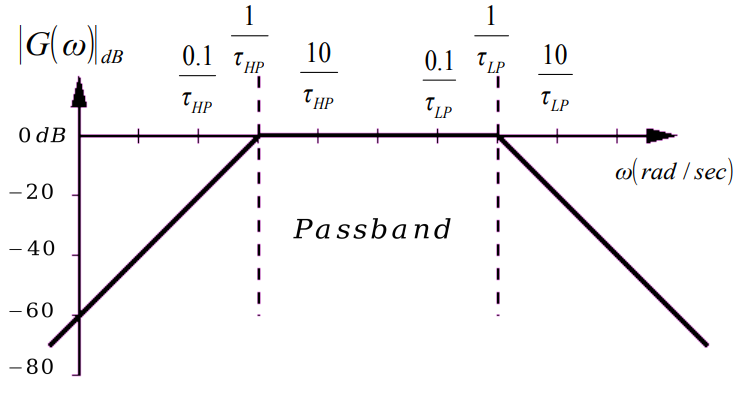
\includegraphics[scale=0.4]{band_pass_filter_amplitude_bode_plot.png}
        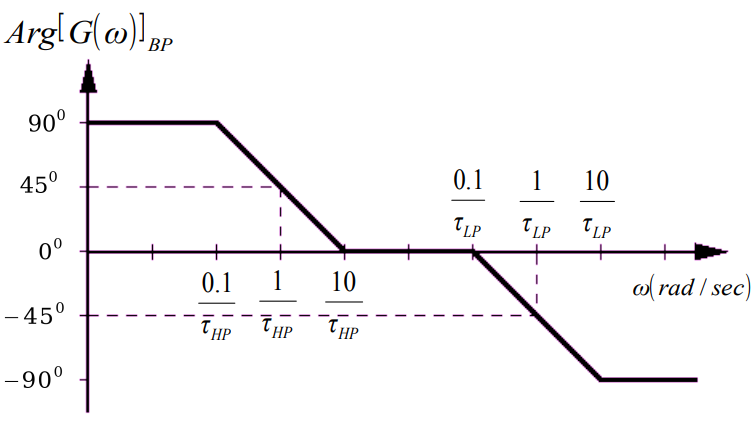
\includegraphics[scale=0.4]{band_pass_filter_phase_bode_plot.png}
        \caption{Band pass filter Bode plots}
        \label{fig:band pass filter}
    \end{figure}
    We would also need a buffer in between the two filters to stop the low pass filter loading the high pass filter.
    Ideally a buffer has high input impedance and no output impedance.
    
    \subsection{Transistor Circuits}
    The circuit in figure \ref{fig:potential divider second voltage source} can be modelled by the circuit in figure \ref{fig:amplifier model} where the amplifier \(G\) has gain \(A_V\approx R_C/R_E\) and \(R_\text{in}\approx (\beta + 1)R_E\) and \(R_\text{out} = R_C\).
    In reality all circuits have some input and output capacitance which can be modelled as shown in figure \ref{fig:amplifier model with capacitors} with \(C_L\) as the output capacitance.
    The transfer function for this circuit is
    \[G(\omega) = A_V\left[\frac{1}{1 + j\omega \tau_\text{LP}}\right]\left[\frac{j\omega\tau_\text{HP}}{1 + j\omega\tau_\text{HP}}\right]\]
    This is similar to a band pass filter but now with gain \(A_V\).
    All that this does is shift the amplitude response up by \(A_V\) (measured in decibels) and leaves the phase response unaffected.
    
    \section{Feedback}
    
    Feedback is the process of sampling part of the output signal and applying it back to the input.
    It may be used to change the a parameter of an amplifier such as gain.
    Negative feedback (inverting the output before applying it to the input) tends to stabilise a process by reducing the output when it gets too large.
    Positive feedback tends to cause rapid changes.
    This is useful in operators and comparator circuits but in general is less useful than negative feedback.
    
    \begin{figure}[ht]
        \centering
        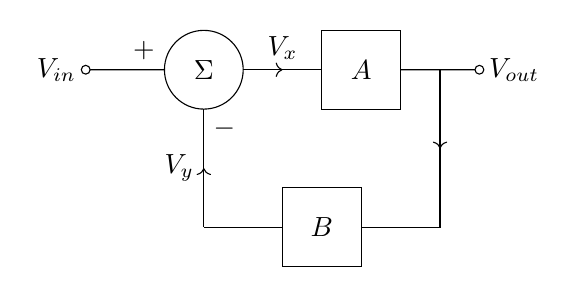
\begin{tikzpicture}
            %\draw[lightgray] (0, 0) grid (5, 5);
            \draw (0, 3) to[short, o-] (1, 3) node[left] at (0, 3) {\(V_\text{in}\)};
            \draw (1.5, 3) circle (0.5);
            \node at (1.5, 3) {\(\Sigma\)};
            \draw (2, 3) -- (3, 3);
            \draw (3, 3.5) rectangle (4, 2.5);
            \node at (3.5, 3) {\(A\)};
            \draw (4, 3) to[short, -o] (5, 3) node[right] at (5, 3) {\(V_\text{out}\)};
            \draw (1.5, 2.5) -- (1.5, 1);
            \draw (1.5, 1) -- (2.5, 1);
            \draw (2.5, 1.5) rectangle (3.5, 0.5);
            \node at (3, 1) {\(B\)};
            \draw (3.5, 1) -- (4.5, 1) -- (4.5, 3);
            \draw[->] (2, 3) -- (2.5, 3);
            \node[above] at (2.5, 3) {\(V_x\)};
            \draw[->] (1.5, 1) -- (1.5, 1.75);
            \node[left] at (1.5, 1.75) {\(V_y\)};
            \draw[->] (4.5, 3) -- (4.5, 2);
            \node[above left] at (1, 3) {\(+\)};
            \node[below right] at (1.5, 2.5) {\(-\)};
        \end{tikzpicture}
        \caption{Feedback circuit}
        \label{fig:feedback circuit}
    \end{figure}
    Figure \ref{fig:feedback circuit} shows a negative feed back circuit. 
    The component \(\Sigma\) is a summing circuit, in this case it is adding the voltage \(V_\text{in}\) and subtracting the voltage \(V_y\).
    \(A\) and \(B\) are circuits with gains \(A\) and \(B\) respectively.
    \(A\) is the main amplifying circuit and \(B\) is the feedback circuit.
    By applying the amplifications to the inputs we see
    \[AV_x = V_\text{out}\qquad \& \qquad BV_\text{out} = V_y\]
    From the summing circuit we get
    \[V_x = V_\text{in} - V_y = V_\text{in} - BV_\text{out}\]
    \[V_\text{out} = A(V_\text{in} - BV_\text{out})\]
    \[\frac{V_\text{out}}{V_\text{in}} = \frac{A}{1 + AB}\]
    As \(B\to 0\) (ie no feedback) \(V_\text{out}/V_\text{in}\to A\).
    As \(A\to \infty\) the transfer function \(V_\text{out}/V_\text{in}\to 1/B\).
    
    Loop gain is the gain from the amplifier input through the amplifier and feedback circuits and back to the amplifier input.
    The loop gain is \(AB\).
    The feedback network is normally just resistive so has no affect on the phase.
    An op-amp has a frequency response so there is a phase shift through the amplifier.
    We assume a \SI{180}{\SIUnitSymbolDegree} phase shift through the amplifier.
    Around the whole loop there is a \SI{-180}{\SIUnitSymbolDegree} phase shift through the amplifier and a \(\SI{180}{\SIUnitSymbolDegree}\) phase shift through the subtracter so there is no overall phase shift.
    This means that what looked like negative feedback is actually positive.
    
    We assume a small signal at the input to \(A\) with a frequency such that the op-amp phase shift is \SI{180}{\SIUnitSymbolDegree}.
    This signal goes round the loop and is multiplied by \(|AB|\).
    It then goes round the loop again and is multiplied by \(|AB|\) again so has now been multiplied by \(|AB|^2\).
    This continues for \(n\) times round the loop the signal has a voltage \(|AB|^n\) times the voltage \(V_\text{signal}\) it started with.
    There are three possibilities for what this means:
    \begin{itemize}
        \item \(|AB|>1\) \(V_\text{signal}\to \infty\). The signal swamps all others, stuff will start overheating and blowing up. The system is said to be unstable.
        \item \(|AB|<1\) \(V_\text{signal}\to 0\). The signal dies away, the system is stable.
        \item \(|AB| = 1\) \(V_\text{signal}\to V_\text{signal}\). This is unlikely unless by design (eg in an oscillator where we just want to keep the original signal)
    \end{itemize}

    \subsection{Measures of Stability}
    There are two widely used measures of stability.
    The first is gain margin.
    To calculate gain margin find the frequency \(\omega_0\) at which the phase shift through the amplifier is exactly \SI{-180}{\SIUnitSymbolDegree}.
    Calculate \(|A(\omega_0)B|\) where \(A(\omega_0)\) is the gain in the amplifier at frequency \(\omega_0\).
    Convert to decibels \(|A(\omega_0)B|_{\si{dB}}\).
    The gain margin is defined as \(-|A(\omega_0)B|_{\si{dB}}\).
    That is the amount by which \(|A(\omega_0)B|_{\si{dB}}\) is less than \SI{0}{dB}.
    If the gain margin is negative then the linear gain is greater than one and the system is unstable, if the gain margin is positive then the linear gain is less than one and the system is stable.
    
    The second measure of stability is phase margin \(\varphi_m\).
    Find a frequency where loop gain \(|AB|\) is \SI{0}{dB} then measure the phase shift through the amplifier.
    Note that phase shift starts at \SI{0}{\SIUnitSymbolDegree} and becomes increasingly negative.
    The amount by which the phase shift at this frequency is greater than \SI{-180}{\SIUnitSymbolDegree} is the phase margin.
    If \(\varphi_m > 0\) the system is stable and if \(\varphi_m < 0\) the system is unstable.
    \[\varphi_m = \arg(A(\omega_0)B) - (-\SI{180}{\SIUnitSymbolDegree}) = \arg(A(\omega_0)B) + \SI{180}{\SIUnitSymbolDegree}\]
    where \(\omega_0\) is a frequency such that
    \[20\log_{10}|A(\omega_0)B| = \SI{0}{dB}\]
    
    The magnitude and phase of the loop gain determines the system stability.
    In a typical circuit the feedback is purely resistive and therefore doesn't change the phase.
    This means that the frequency at which the phase of the loop reaches \SI{-180}{\SIUnitSymbolDegree} depends only on the op-amp gain \(A\) which is outside of our control.
    
    To maximise gain margin (make the system more stable) we want to minimise the gain at \(\omega_0\).
    Since \(A\) is outside of our control the maximum gain margin comes with minimum values of \(B\).
    Conversely the worst system stability comes with the maximum value of \(B\).
    Potentially the voltage follower (apply the output of an op-amp directly back to \(V_-\)) is the most unstable op-amp circuit as it uses 100 \% feedback.
    
    \subsection{Op-amp Frequency Response}
    An op-amp can be thought of as three sections:
    \begin{enumerate}
        \item Differential stage: some gain, subtraction of \(V_+\) and \(V_-\).
        \item Gain stage: high gain, high output impedance.
        \item Output stage: low output impedance.
    \end{enumerate}
    Each stage has a frequency response.
    Each frequency response is first-order low pass with a different cut off frequency for each stage.
    The cut off frequencies are similar for the differential and gain stages.
    The Bode plots for the individual stages are shown in figure \ref{fig:op-amp bode plot individual} and combined for the whole op-amp in figure \ref{fig:op-amp bode plot combined} where the op-amp is configured to use 100 \% feedback.
    
    \begin{figure}[ht]
        \centering
        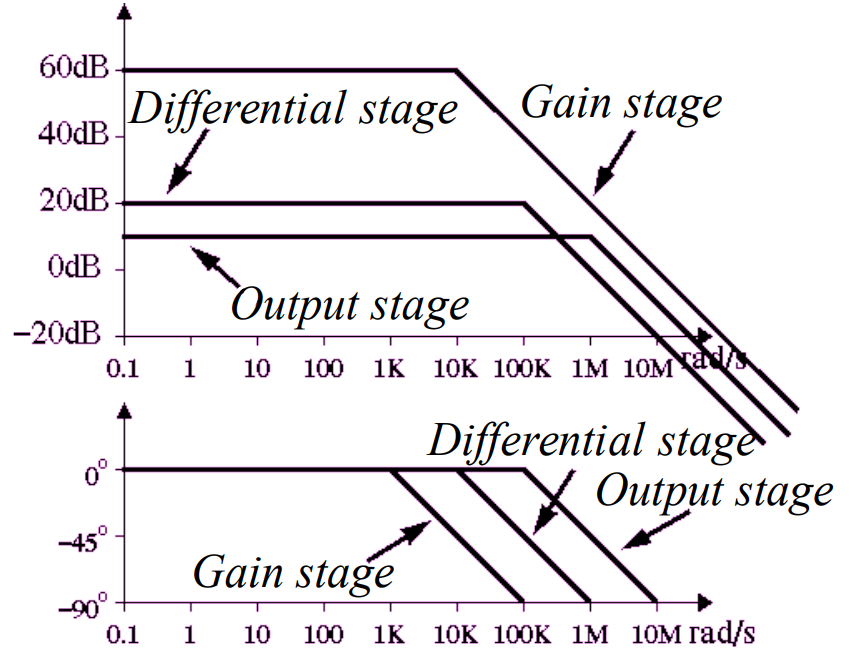
\includegraphics[scale=0.35]{op-amp_bode_plot_individual.png}
        \caption{Bode plots for each stage of an op-amp}
        \label{fig:op-amp bode plot individual}
    \end{figure}

    \begin{figure}[ht]
        \centering
        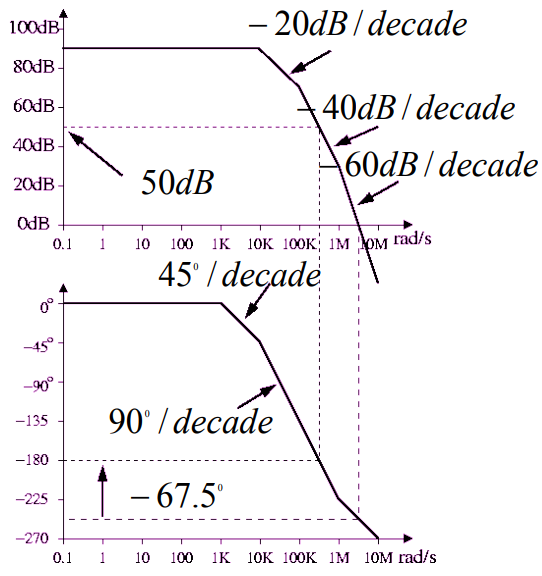
\includegraphics[scale=0.45]{op-amp_bode_plot_combined.png}
        \caption{Bode plots for each stage of an op-amp}
        \label{fig:op-amp bode plot combined}
    \end{figure}
    
    The precise values of the cut off frequencies depend on the circuit but for the Bode plots shown the gain margin is \SI{-50}{dB} and the phase margin is \SI{-67.5}{\SIUnitSymbolDegree}, both are negative so the op-amp on its own is unstable and therefore requires compensation.
    
    \section{Op-amp Compensation}
    The simplest compensation that we can use for an op-amp is to add a low pass filter to the output with the resistance and capacitance such that the overall circuit has the desired gain/phase margin.
    
    For example if we want a phase margin of \SI{60}{\SIUnitSymbolDegree} then we need a phase shift of \SI{-120}{\SIUnitSymbolDegree} (ie \SI{60}{\SIUnitSymbolDegree} above \SI{-180}{\SIUnitSymbolDegree}).
    The op-amp stages all have high cut off frequencies so it is fair to assume that the filter will have the lowest cut off frequency.
    The filter introduces a \SI{-90}{\SIUnitSymbolDegree} phase shift so we need to find a frequency at which the phase shift of the op-amp stages is \SI{-30}{\SIUnitSymbolDegree} (ie \SI{90}{\SIUnitSymbolDegree} above the desired phase shift of \SI{-120}{\SIUnitSymbolDegree}).
    We do this by looking at the phase shift Bode plot for the op-amp stages in figure \ref{fig:op-amp bode plot combined} and we see that this gives us a frequency of approximately \(\SI{4600}{rad.s^{-1}}\).
    We need the gain at this point to be \SI{0}{dB} so that this is the point at which we measure the phase shift to get the phase margin.
    To do this we draw a line through the point at \(\SI{4600}{rad.s^{-1}}\) and \SI{0}{dB} and we see the frequency at which it intersects the amplitude response Bode plot of the op-amp stages.
    This frequency \(\omega_c\) is the frequency that we want our low pass filter to cut off at.
    So we need \(1/\tau = \omega_c\implies RC = 1/\omega_c\).
    
    All op-amps require some form of compensation and there are slightly better ways to do this that don't create such a low cut off for the op-amp but this is definitely the simplest way to do it.
    The frequency response is first order low pass at least up to frequency where the open loop gain \(A_{ol}\) falls to unity.
    The open loop gain is a constant \(A_{ol}(\text{DC})\) (the open loop gain for DC) times a low pass term:
    \[A_{ol} = \frac{A_{ol}(\text{DC})}{1 + j\omega/\omega_c}\]
    Note that \(1/\omega_c = \tau\).
    The unity gain bandwidth is the frequency \(\omega_{ug}\) at which \(A_{ol}(\omega_{ug}) = 1\)
    \[\A_{ol}(\omega_{ug}) = \frac{A_{ol}(\text{DC})}{1 + j\omega_{ug}/\omega_c} = 1\]
    \(\omega_{ug}\) is high so \(\omega_{ug} \approx A_{ol}\omega{c}\)
    
    \subsection{Op-amp With Feedback}
    \begin{figure}[ht]
        \centering
        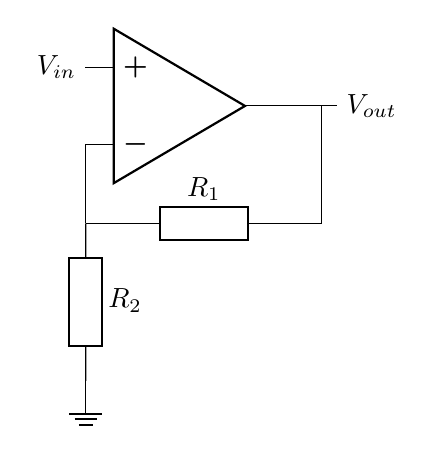
\begin{tikzpicture}
            %\draw[lightgray] (0, 0) grid (5, 5);
            \node[op amp, yscale=-1] (opamp) at (2, 4) {};
            \node[left] at (opamp.+) {\(V_\text{in}\)};
            \draw (opamp.-) -- ($(opamp.-)+(0, -1)$);
            \draw ($(opamp.-)+(0, -1)$) to[R=\(R_2\)] ($(opamp.-)+(0, -3)$);
            \node[ground] at ($(opamp.-)+(0, -3)$) {};
            \draw ($(opamp.-)+(0, -1)$) to[R=\(R_1\)] ($(opamp.-)+(3, -1)$);
            \draw ($(opamp.-)+(3, -1)$) -- ($(opamp.-)+(3, 0.49)$);
            \draw (opamp.out) -- (4, 4) node[right] at (4, 4) {\(V_\text{out}\)};
        \end{tikzpicture}
        \caption{An op-amp with feedback}
        \label{fig:op-amp with feedback}
    \end{figure}
    Consider the circuit shown in figure \ref{fig:op-amp with feedback}.
    What is the transfer function of this circuit?
    
    The feedback voltage is given by
    \[V_\text{out}\frac{R_2}{R_1 + R_2} = V_{\text{in}-}\]
    using the op-amp rule that \(V_{\text{in}+} = V_{\text{in}-} = V_\text{in}\) we get
    \[V_\text{in} = V_\text{out}\frac{R_2}{R_1 + R_2}\]
    \[\frac{V_\text{out}}{V_\text{in}} = \frac{R_1 + R_2}{R_2}\]
    We can use the gain equation \(V_\text{out} = A(V_{\text{in}+} - V_{\text{in}-})\), where \(A = A_{ol}(\omega)\), to get
    \[V_\text{out}(\omega) = \frac{A_{ol}(\text{DC})}{1 + j\omega\tau}\left[V_\text{in} - \frac{R_2}{R_1 + R_2}V_\text{out}\right]\]
    \[\frac{V_\text{out}}{V_\text{in}} = \frac{A_{ol}(\text{DC})(R_1 + R_2)}{(1 + j\omega\tau)(R_1 + R_2) + A_{ol}(\text{DC})R_2} = \frac{R_1 + R_2}{R_2}\left[ \frac{1}{1 + \frac{R_1 + R_2}{A_{ol}(\text{DC})R_2}(1 + j\omega\tau)}\right]\]
    At low frequencies the \(A\) term dominates and \(V_\text{out}/V_\text{in}\approx 1\). 
    At high frequencies the \(j\omega\tau\) term dominates.
    The 1 in the \(1 + j\omega\tau\) can be neglected.
    This gives the approximation
    \[\frac{V_\text{out}}{V_\text{in}}\approx \frac{R_1 + R_2}{R_2}\left[\frac{1}{1 + \frac{R_1 + R_2}{A_{ol}(\text{DC})R_2}j\omega\tau}\right]\]
    This is a first order low pass filter times a constant and this can be shown by writing it as
    \[\frac{V_\text{out}}{V_\text{in}}\approx k\left[\frac{1}{1 + j\omega\tau'}\right]\]
    where
    \[k = \frac{R_1 + R_2}{R_2}\quad\text{and}\quad \tau' = \frac{R_1 + R_2}{A_{ol}(\text{DC})R_2}\tau\]
    \begin{figure}[ht]
        \centering
        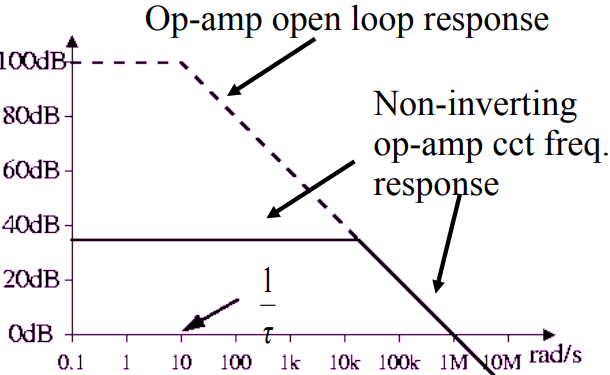
\includegraphics[scale=0.4]{op-amp_non_inverting_bode_plot.png}
        \caption{The amplitude response Bode plot of a non-inverting op-amp like in figure \ref{fig:op-amp with feedback}}
    \end{figure}

    \section{More Op-amp Circuits and Filters}
    \subsection{Differentiator Op-amp}
    \begin{figure}[ht]
        \centering
        \begin{tikzpicture}
            \node[op amp](opamp) at (0, 0) {};
            \draw (opamp.-) to[C=\(C\), -o] ($(opamp.-)+(-2, 0)$) node[left] at ($(opamp.-)+(-2, 0)$) {\(V_\text{in}\)};
            \draw (opamp.+) -- ($(opamp.+)+(0, -1)$) node[ground] at ($(opamp.+)+(0, -1)$) {};
            \draw (opamp.-) -- ($(opamp.-)+(0, 1)$) to[R=\(R\)] ($(opamp.-)+(2.5, 1)$) -- ($(opamp.-)+(2.5, -0.49)$);
            \draw (opamp.out) to[short, -o] ($(opamp.out)+(1, 0)$) node[right] at ($(opamp.out)+(1, 0)$) {\(V_\text{out}\)};
        \end{tikzpicture}
        \caption{A differentiator op-amp}
        \label{fig:differentiator op-amp}
    \end{figure}
    Figure \ref{fig:differentiator op-amp} shows a differentiator op-amp.
    We can perform nodal analysis to find the transfer function and split it into standard functions:
    \[\frac{V_\text{in}}{1/j\omega C} + \frac{V_\text{out}}{R} = 0\]
    \[\frac{V_\text{out}}{V_\text{in}} = -j\omega RC = [j\omega][-\tau]\]
    The term \(j\omega\) gives a amplitude response Bode plot that is a straight line with a gradient of \SI{20}{dB}/decade through \SI{0}{dB}, \(\SI{1}{rad.s^{-1}}\).
    The constant term gives an offset of \(-\tau\,\si{rad.s^{-1}}\).
    The Bode plot for this circuit is shown in figure \ref{fig:differentiator op-amp bode plot}
    \begin{figure}[ht]
        \centering
        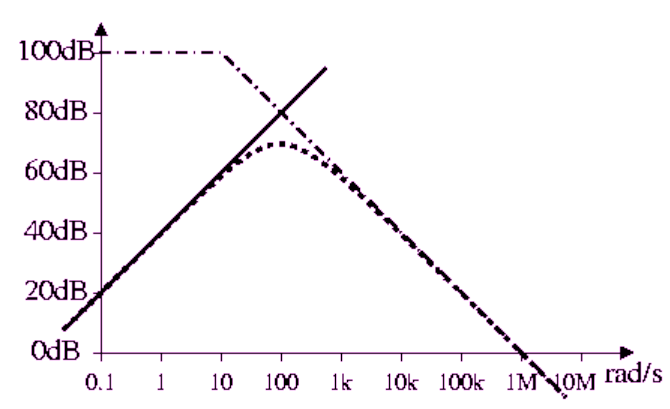
\includegraphics[scale=0.4]{op-amp_differentiatior_bode_plot.png}
        \caption{Differentiator op-amp amplitude response Bode plot}
        \label{fig:differentiator op-amp bode plot}
    \end{figure}
    
    \subsection{Filters}
    A filter is a frequency selective device which passes certain frequencies and attenuates others.
    There are four common classifications of filters:
    \begin{enumerate}
        \item Low pass - passes low frequencies and blocks higher ones
        \item High pass - passes high frequencies and blocks lower ones
        \item Band pass - passes a band of frequencies and blocks those higher or lower than the band
        \item Band reject - blocks a band of frequencies and passes those higher or lower than the band
    \end{enumerate}
    An active filter (as opposed to a passive filter) uses an active component, that is a component capable of adding power to the circuit such as an op-amp.
    
    In the filter pass band the voltage gain \(V_\text{out}/V_\text{in}\) is never more than \SI{3}{dB} below the maximum gain.
    At the passband edges exactly one half of the maximum power is transmitted.
    The filter band with is measured between the frequencies at which the gain is exactly \SI{3}{dB} less than the maximum.
    A low pass filter has a band width from DC to the passband edge.
    The pass band is not defined for a high pass filter.
    
    When designing an active filter with an op-amp first check that the op-amp has enough gain.
    Usually we want to ensure a minimum safety margin of \SI{20}{dB} gain margin.
    To do this we draw a Bode plot of the desired filter response and the op-amp's open loop frequency response.
    
    Another standard response is an integrator op-amp.
    This can be made using the circuit in figure \ref{fig:integrator op-amp}.
    \begin{figure}[ht]
        \centering
        \begin{tikzpicture}
        \node[op amp](opamp) at (0, 0) {};
        \draw (opamp.-) to[R=\(R\), -o] ($(opamp.-)+(-2, 0)$) node[left] at ($(opamp.-)+(-2, 0)$) {\(V_\text{in}\)};
        \draw (opamp.+) -- ($(opamp.+)+(0, -1)$) node[ground] at ($(opamp.+)+(0, -1)$) {};
        \draw (opamp.-) -- ($(opamp.-)+(0, 1)$) to[C=\(C\)] ($(opamp.-)+(2.5, 1)$) -- ($(opamp.-)+(2.5, -0.49)$);
        \draw (opamp.out) to[short, -o] ($(opamp.out)+(1, 0)$) node[right] at ($(opamp.out)+(1, 0)$) {\(V_\text{out}\)};
        \end{tikzpicture}
        \caption{A integrator op-amp}
        \label{fig:integrator op-amp}
    \end{figure}
    \[\frac{V_\text{out}}{V_\text{in}} = \frac{-1}{j\omega RC}\]
    An integrator op-amp has an amplitude frequency response Bode plot of a straight line through \SI{0}{dB} and \(1/\tau\,si{rad.s^{-1}}\) which has gradient of \SI{-20}{dB}/decade.
    
    \section{Op-amp Performance}
    There is a collection of ways that we measure op-amp performance and which metrics we use depends on what is most important for the circuit we are designing.
    Some of these are shown in table \ref{tab:op-amp metrics} along with the ideal values that these metrics would have and a reasonable practical value.
    \begin{table}[ht]
        \centering
        \begin{tabular}{c|c|c}
            Parameter & Ideal Value & Practical Value\\ \hline
            &&\\[-0.3cm]
            Gain & \(\infty\) & \(\num{2e5} = \SI{106}{dB}\)\\
            Input current & 0 & \SI{80}{nA}\\
            Bandwidth & \(\infty\) & \SI{0}{dB} open loop gain at \SI{1}{MHz}\\
            Output voltage range & Unlimited & Power supply minus \SI{2}{V}\\
            Output impedance & 0 & \SI{75}{\ohm}\\
            Power consumption & 0 & \SI{50}{mW}\\
            Slew rate & \(\infty\) & \SI{0.5}{V/\micro s}\\
            Common mode rejection ratio & \(\infty\) & \SI{90}{dB}\\
            Power supply rejection ratio & \(\infty\) & \SI{30}{\micro V/V}\\
            Input offset voltage & 0 & \SI{2}{mV}
        \end{tabular}
        \caption{Op-amp metrics}
        \label{tab:op-amp metrics}
    \end{table}
    The gain is the open loop gain of the op-amp without any feedback.
    It is the parameter \(A\) in the equation
    \[V_\text{out} = A(V_+-V_-)\]
    Ideally it is infinite but this isn't practical so we settle for a large value.
    \(A > \SI{100}{dB}\) is easily achieved at low frequencies (eg for a 741C op-amp \(A = \SI{106}{dB}\)).
    
    The input current should be 0 (as stated in the golden rules of op-amps).
    This is reached by having large input impedances of greater than \SI{10e18}{\ohm} in MOSFET devices or \SI{10e6}{\ohm} in bipolar transistor devices.
    The 741C has a bipolar transistor input stage and has an input current of \SI{80}{nA}.
    
    An ideal op-amp would work with DC \((\SI{0}{Hz})\) up to infinite frequencies.
    In reality the 741C has a cut off at \SI{10}{Hz} and after that gain falls at 20 dB/decade.
    This gives it a unity bandwidth of \SI{1}{MHz}
    
    If we use the equation
    \[V_\text{out} = A(V_+-V_-)\]
    with \(A = \num{2e5}\) and \(V_+-V_- = \SI{3.5}{V}\) then we would need \(V_\text{out} = \SI{700}{kV}\).
    This is far too high.
    In reality the actual output voltages possible is limited by the power supply and the output swing capability of the op-amp.
    This results in a maximum voltage of about \SI{2}{V} less than the power supply.
    
    Ideally the output should be like a voltage source (so no output impedance) this isn't possible.
    The output impedance of the 741C is \SI{75}{\ohm} and in general we want it less than \SI{100}{\ohm}.
    
    We would like power consumption to be zero.
    This isn't possible but it can be low.
    Op-amps that consume only a few micro watts are possible.
    The 741C consumes \SI{50}{mW}.
    
    The op-amp output voltage can't change instantaneously even if the input can.
    The slew rate is defined as the the maximum voltage change per unit time when the op-amp is in a voltage follower mode (\SI{100}{\%} negative feedback).
    We would like the slew rate to be as high as possible.
    For the 741C it is \SI{0.5}{V/\micro s}.
    In general values under \SI{20}{V/\micro s} are good.
    Slew rate is a large signal phenomenon only.
    
    In differencing mode an op-amp amplifies the difference between two inputs by \(A_{DM}\).
    In common mode the two inputs are the same so the difference should be 0 so the output should be 0 and the gain \(A_{CM}\) should be 0.
    However this isn't what we see.
    In general we want \(A_{CM}\ll 1\).
    We define the common mode rejection ratio as
    \[20\log_{10}\left(\frac{A_{DM}}{A_{CM}}\right)\]
    For a 741C this is \SI{90}{dB}.
    We would like it to be infinite.
    
    We define the power supply rejection ratio as the change in output voltage per unit change in power supply voltage.
    It is a measure of how noise in the power supply effects the output.
    Ideally we want it to be 0.
    In practice for a 741C it is \SI{30}{\micro V/V}
    
    If \(V_+=V_-\) the output should be 0 but it isn't due to imbalances within the op-amp.
    We can fix this by applying a voltage to the non-inverting input such that the output is 0.
    Ideally we would like not to do this so we want the offset voltage to be 0.
    
    \subsection{Amplifier Classification}
    There are various types of amplifier.
    Some of them are:
    \begin{itemize}
        \item Voltage amplifier. Gain is output voltage divided by input voltage.
        \[\text{gain} = \frac{V_\text{out}}{V_\text{in}}\]
        gain is dimensionless.
        \item Current amplifier. Gain is input current divided by input current.
        \[\text{gain} = \frac{I_\text{out}}{I_\text{in}}\]
        Gain is dimensionless.
        \item Transresistance amplifier. Gain is output voltage divided by input current.
        \[\text{gain} = \frac{V_\text{out}}{I_\text{in}}\]
        Gain is measured in ohms.
        \item Transconductance amplifier. Gain is output current divided by input voltage.
        \[\text{gain} = \frac{I_\text{out}}{V_\text{in}}\]
        Gain is measured in siemens.
    \end{itemize}
\end{document}
